% Sablon pentru realizarea lucrarii de licenta, conform cu recomandarile
% din ghidul de redactare:
% - https://fmi.unibuc.ro/finalizare-studii/
% - https://drive.google.com/file/d/1xj9kZZgTkcKMJkMLRuoYRgLQ1O8CX0mv/view

% Multumiri lui Gabriel Majeri, acest sablon a fost creat pe baza
% codului sursa a lucrarii sale de licenta. 
% Codul sursa: https://github.com/GabrielMajeri/bachelors-thesis
% Website: https://www.gabrielmajeri.ro/
%
% Aceast sablon este licentiat sub Creative Commons Attribution 4.0 International License.

% !TEX program = xelatex

\documentclass[12pt, a4paper]{report}

\bibliographystyle{alpha}

% Suport pentru diacritice și alte simboluri
\usepackage{fontspec}

% Suport pentru mai multe limbi
\usepackage{polyglossia}

% Setează limba textului la română
\setdefaultlanguage{romanian}
% Am nevoie de engleză pentru rezumat
\setotherlanguages{english}

% Indentează și primul paragraf al fiecărei noi secțiuni
\SetLanguageKeys{romanian}{indentfirst=true}

% Suport pentru diferite stiluri de ghilimele
\usepackage{csquotes}

\DeclareQuoteStyle{romanian}
  {\quotedblbase}
  {\textquotedblright}
  {\guillemotleft}
  {\guillemotright}

% Utilizează biblatex pentru referințe bibliografice
\usepackage[
    maxbibnames=50,
    sorting=nty
]{biblatex}

\addbibresource{bibliography.bib}

% Setează spațiere inter-linie la 1.5
\usepackage{setspace}
\onehalfspacing

% Modificarea geometriei paginii
\usepackage{geometry}
\usepackage[absolute,overlay]{textpos}

% Include funcțiile de grafică
\usepackage{graphicx}
% Încarcă imaginile din directorul `images`
\graphicspath{{./images/}}

% Listări de cod
\usepackage{listings}

% Linkuri interactive în PDF
\usepackage[
    colorlinks,
    linkcolor={black},
    menucolor={black},
    citecolor={black},
    urlcolor={blue}
]{hyperref}

\usepackage{mathtools}
% Simboluri matematice codificate Unicode
\usepackage[warnings-off={mathtools-colon,mathtools-overbracket}]{unicode-math}

% Comenzi matematice
\usepackage{amsmath}
\usepackage[table]{xcolor}
\usepackage{tabularx}
\usepackage{subcaption}
\usepackage{float}
\usepackage[section]{placeins}

% Formule matematice
\newcommand{\bigO}[1]{\symcal{O}\left(#1\right)}
\DeclarePairedDelimiter\abs{\lvert}{\rvert}

% Suport pentru rezumat în două limbi
% Bazat pe https://tex.stackexchange.com/a/70818
\newenvironment{abstractpage}
  {\cleardoublepage\vspace*{\fill}\thispagestyle{empty}}
  {\vfill\cleardoublepage}
\renewenvironment{abstract}[1]
  {\bigskip\selectlanguage{#1}%
   \begin{center}\bfseries\abstractname\end{center}}
  {\par\bigskip}

% Suport pentru anexe
\usepackage{appendix}

% Stiluri diferite de headere și footere
\usepackage{fancyhdr}

% Metadate
\title{Detectarea tranzacţiilor bancare frauduloase utilizând învăţare automată
nesupervizată}
\author{Eftimie Petre-Laurenţiu}

% Generează variabilele cu @
\makeatletter

\begin{document}

% Front matter
\cleardoublepage
\let\ps@plain

% Pagina de titlu
\begin{titlepage}

% Redu marginile
\newgeometry{left=2cm,right=2cm,bottom=1cm}

\begin{figure}[!htb]
    \centering
    \begin{minipage}{0.2\textwidth}
        
\includegraphics[width=\linewidth]{logo-ub.png}
    \end{minipage}
    \begin{minipage}{0.5\textwidth}
        \large
        \vspace{0.2cm}
        \begin{center}
            \textbf{UNIVERSITATEA DIN BUCUREȘTI}
        \end{center}
        \vspace{0.3cm}
        \begin{center}
            \textbf{
                FACULTATEA DE \\
                MATEMATICĂ ȘI INFORMATICĂ
            }
        \end{center}
    \end{minipage}
    \begin{minipage}{0.2\textwidth}
        
\includegraphics[width=\linewidth]{logo-fmi.png}
    \end{minipage}
\end{figure}

\begin{center}
\textbf{SPECIALIZAREA INFORMATICĂ}
\end{center}

\vspace{1cm}

\begin{center}
\Large \textbf{Lucrare de licență}
\end{center}

\begin{center}
\huge \textbf{\MakeUppercase{\@title}}
\end{center}

\vspace{3cm}

\begin{center}
\large \textbf{Absolvent \\ \@author}
\end{center}

\vspace{0.25cm}

\begin{center}
\large \textbf{Coordonator științific \\ Conf. dr. Cristian Rusu}
\end{center}

\vspace{2cm}

\begin{center}
\Large \textbf{București, iunie 2024}
\end{center}
\end{titlepage}
\restoregeometry
\newgeometry{
    margin=2.5cm
}

\fancypagestyle{main}{
  \fancyhf{}
  \renewcommand\headrulewidth{0pt}
  \fancyhead[C]{}
  \fancyfoot[C]{\thepage}
}

\addtocounter{page}{1}

% Rezumatul
\begin{abstractpage}

\begin{abstract}{romanian}  

    Detecţia anomaliilor este un subiect ce apare frecvent în cercetarea din 
    domeniul învăţării automate. Acest fapt se datorează multitudinii de 
    aplicaţii într-o gamă largă de industrii. 

    Totuşi, găsirea unei tehnici bune de rezolvare a problemei este
    dificilă în cele mai multe cazuri, 
    întrucât este costisitor sau aproape imposibil să obţii date 
    despre evenimentele rare ce merită semnalate. 

    În această lucrare, explorăm un set de date ce conţine 
    informaţii despre tranzacţii bancare
    folosind 3 algoritmi de învăţare automată nesupervizată:
    "One Class SVM", "Gaussian Mixture Model" şi "Kernel Density Estimation". 
    Performanţa acestora din urmă 
    este comparată prin metricile: "accuracy", "precision", "recall" şi "f1 score".

    Obiectivul este detectarea tranzacţiilor frauduloase.    
\end{abstract}

\begin{abstract}{english}
    
    Anomaly detection is a topic appearing frequently in machine learning research.
    This is due to its many applications in various industrial settings.

    However, finding a good algorithm to solve this problem is difficult 
    in most cases, since obtaining data about rare events that are worth reporting
    is costly or almost impossible.

    In this paper, we analyze a dataset containing information about 
    bank transactions using 3 unsupervised machine learning 
    algorithms: "One Class SVM", "Gaussian Mixture Model" and 
    "Kernel Density Estimation". 
    Their performance is compared using the following metrics: 
    "accuracy", "precision", "recall" and "f1 score".

    Our objective is detecting fraudulent transactions.

\end{abstract}

\end{abstractpage}

\tableofcontents

% Main matter
\cleardoublepage
\pagestyle{main}
\let\ps@plain\ps@main

\chapter{Introducere}

\section{Inteligenţa artificială}

Este un domeniu de studiu din Informatică, discutat încă din prima jumătate a 
secolului al XX-lea, dar care a devenit popular abia la finalul secolului menţionat 
anterior.

Aceasta are ca scop simularea inteligenţei umane folosind diverşi algoritmi şi 
structuri de date. Există mai multe arii de cercetare în acest domeniu, precum: 
raţionamentul, reprezentarea cunoştinţelor, planificarea, procesarea limbajului 
natural, cât şi învăţarea automată care va fi prezentată detaliat în această lucrare.
Totuşi, obiectivul pe termen lung al cercetătorilor este de a simula inteligenţa 
generală, nu doar părţi specifice din aceasta.

Popularitatea acesteia a început să crească odată cu mărirea spaţiului de stocare,
a puterii de procesare, cât şi cu faptul că sistemele de calcul au devenit mai 
accesibile. 

De asemenea, deşi algoritmii existenţi nu s-au mai îmbunătăţit 
semnificativ, accesul la o cantitate enormă de date în ziua de astăzi, anume 
fenomenul "Big Data", a oferit un sprijin considerabil pentru performanţa 
învăţării inteligenţei artificiale\cite{ai-history}.

În acest domeniu, datele colectate, cât şi calitatea lor au un rol extrem de important.
Oricât de bun ar fi algoritmul propus, în lipsa unor date reprezentative pentru 
problema ce trebuie rezolvată, performanţa va fi îndoielnică. Putem spune că datele 
sunt cele care introduc particularităţile din lumea reală în spaţiul teoretic 
al inteligenţei artificiale.

Prin urmare, se observă că aplicabilitatea inteligenţei artificiale 
a fost împiedicată în principal de considerente practice, nu neapărat teoretice.

Printre succesele recente din domeniu se remarcă AlphaFold, un model 
inventat de DeepMind care prezice structura proteinelor din secvenţele 
de amino acizi, GPT-3 al OpenAI ce poate genera text care să răspundă la 
întrebările utilizatorilor aproape ca o fiinţă umană, dar şi algoritmii 
pentru maşini autonome dezvoltaţi de cei de la Tesla.

Utilizarea inteligenţei artificiale poate reduce costurile asociate 
sarcinilor ce ar necesita efortul unei persoane, dar de multe ori apare şi 
problema eticii, precum în cazul înlocuirii recrutorilor cu un program 
ce selectează candidaţii pentru un loc de muncă în funcţie de anumite 
criterii care nu ar fi întocmai corespunzătoare.

Automatizarea detecţiei anomaliior reprezintă una din posibilele aplicaţii
ale inteligenţei artificiale, subiect ce va fi abordat în această lucrare.

\section{Definiţia anomaliilor}


O \textbf{anomalie} este o entitate ce diferă semnificativ de restul enităţilor din 
setul de date. Definiţia lui Hawkins este urmatoarea\cite{hawkins1980identification}:
\textit{"O anomalie este o observaţie ce deviază atât de mult faţă de restul observaţiilor,
încât să creeze suspiciunea că a fost generată de un mecanism diferit"}.

Datele sunt colectate prin observarea unor procese, de preferat din viaţa reală, 
precum funcţionarea
unui motor sau traficul pe o reţea de calculatoare. În majoritatea timpului, procesele
generează date ce corespund unei derulări normale, dar în anumite cazuri acestea se 
comportă anormal şi astfel apar anomaliile. 

\textit{"Normalitatea"} observaţiilor este definită
de oameni. Algoritmii de învăţare automată pot să semnaleze potenţialele
abateri, dar în final, decizia rămâne a omului.

De asemenea, caracteristicile anomaliilor depind de domeniul 
unde acestea apar. Ce este considerat anomalie în domeniul 
medical, va diferi aproape complet de domeniul finanțelor, 
spre exemplu. 

Mai mult, unele observaţii nici măcar nu 
pot reprezenta comportament anormal în afara unui context 
bine definit sau fără a apărea în prezența altor observaţii
care adunate ar forma o anomalie. Un exemplu de comportament
ce poate fi observat în traficul de date pe o rețea al unei 
organizații ar fi 
conectarea de la distanță pe un anumit calculator. Acest lucru
se întâmplă regulat și nu poate ridica nicio suspiciune de 
cele mai multe ori. Dar în combinație cu o oră târzie de 
accesare, când probabil angajații nu mai sunt la lucru, 
sau cu alte comenzi care sunt folosite succesiv pentru a 
comite un atac cibernetic, o observaţie ce în general 
este complet normală, acum prezintă caracteristici anormale.

Prin urmare, se observă că decizia de a eticheta o observaţie ca fiind anomalie 
sau nu este una dificilă chiar şi pentru un om, iar în combinație cu faptul 
că obţinerea de date ce ar putea fi anormale este de cele mai multe ori costisitoare,
face ca evaluarea sistemelor de detecţie să devină una problematică.


\section{Avantajele învăţării automate}

Când sarcinile ce trebuie îndeplinite periodic, necesare bunei funcţionări a unei 
companii spre exemplu, încep să ocupe o mare parte din timpul oamenilor, apare 
nevoia automatizării. 

În general, soluţiile ce includ stabilirea unui set de reguli
sunt de preferat, datorită simplităţii lor. Un exemplu banal ar fi verificarea 
siguranţei unei parole introduse de utilizator la crearea unui cont pe o platformă
web. Este suficient să verificăm dacă parola are un număr minim precizat de caractere 
sau dacă conţine anumite simboluri ce reduc vulnerabilitatea în faţa unui atac cibernetic.

Din păcate, multe din problemele cu care ne confruntăm nu au soluţii simple, 
iar 
în unele situaţii, problema este greu de definit, mai ales în lipsa exemplelor, precum 
este cazul detecţiei anomaliilor.
Aici intervine învăţarea automată ce încearcă să aproximeze posibilul set de reguli, 
prea complex pentru a fi definit, ce ar putea rezolva problema. Am putea spune că 
această tehnică "învaţă" setul de reguli 
din datele puse la dispoziţie, de unde şi denumirea. Evident, o aproximare 
nu are cum să fie perfectă, dar este suficient de bună încât să scutească oamenii de 
o mare parte din treabă. În cazul tranzacţiilor bancare, 
ce s-au efectuat în medie 
de 1.98 de miliarde pe zi la nivel global în 2023\cite{transactions-per-day}, 
nu este greu de observat că verificarea manuală
de către oameni este imposibilă, iar găsirea unui set simplu de reguli care să 
le caracterizeze din nou este o problemă dificilă. Totuşi, învăţarea automată 
ne poate ajuta să minimizăm fraudele ce trec nedetectate de la milioane la câteva zeci
pe zi.

\section{Caracterizarea anomaliilor nu este viabilă}

Un exemplu ce ilustrează de ce obţinerea de informaţii
despre anomalii este costisitoare ar putea fi activitatea unui
motor defect.

În acest caz, avem 2 variante:
\begin{itemize}
    \item Una dintre ele 
        este să \textbf{simulăm} 
        într-un fel sau altul comportamentul unui motor defectuos, dar 
        se observă că această operaţiune este greu de realizat şi chiar dacă am reuşi 
        să o ducem la capăt, datele colectate nu ar fi autentice şi ar putea duce 
        la o reprezentare incorectă a anomaliilor. 
        De asemenea, simularea
        sabotajului ar necesita identificarea unui algoritm corespunzător, 
        dar acest lucru ar duce de fapt la rezolvarea problemei iniţiale.

    \item A doua variantă implică \textbf{sabotarea 
        intenţionată} a motorului pentru a obţine datele, dar acest lucru produce un 
        cost prea mare de cele mai multe ori. 
\end{itemize}

Este evident că definirea anomaliei în acest context nu este viabilă, iar 
cazul nu este singular. Tranzacţiile frauduloase ce constituie tema acestei lucrări 
suferă de aceleaşi probleme, ba mai mult, nici măcar nu avem opţiunea de a 
sabota intenţionat derularea normală a tranzacţiilor. De asemenea,
dacă anomaliile apar ca urmare a unor acțiuni cu caracter maliţios,
atunci adversarii responsabili pentru acestea vor încerca să 
evite mecanismele existente de detecţie prin schimbarea 
frecventă a metodelor folosite. Prin urmare, ce era considerat
comportament normal înainte, acum poate indica prezența unui 
atac.


În schimb, 
este mult mai uşor şi cel mai probabil 
implică un cost aproape inexistent, să urmărim activitatea unui motor 
în stare bună de funcţionare şi să folosim datele respective pentru a 
defini ce înseamnă o observaţie normală.

\section{Aplicaţii ale detecţiei anomaliilor}

În aproape toate domeniile apare problema semnalării unor fenomene sau evenimente 
ieşite din comun ce necesită atenţia unei persoane pentru analiză. Mai jos prezentăm
doar câteva din cazurile unde detecţia anomaliilor este necesară, cât şi ce ar 
reprezenta o anomalie pentru fiecare:

\begin{itemize}
    \item \textbf{Fraude financiare}: ne dorim să semnalăm comportamentul ciudat 
    observat într-o serie de tranzacţii, precum activitatea generată de 
    o persoană care foloseşte cardul de credit al altei persoane în mod 
    neautorizat. Această aplicaţie constituie şi obiectul lucrării noastre\cite{financial-fraud}.
    \item \textbf{Intruziune în reţele de calculatoare}: vrem să semnalăm activitatea
    neobişnuită ce poate indica un potenţial atac cibernetic sau accesul 
    neautorizat al unui terţ maliţios\cite{network-traffic}.
    \item \textbf{Controlul calităţii în procesele de fabricaţie}: suntem interesaţi să monitorizăm 
    procesul de producţie pentru a raporta eventualele defecţiuni ce ar afecta 
    calitatea produsului\cite{quality-control}.
    \item \textbf{Domeniul medical}: vrem să identificăm anomalii în analizele de sânge, 
    semnele vitale sau imaginile medicale ale pacientului pentru a depista şi preveni
    anumite afecţiuni\cite{medical-images}.
    \item \textbf{Reţele sociale}: ne dorim să raportăm automat conţinutul postat ce 
    poate include remarci jignitoare, precum comentariile rasiste sau xenofobe,
    astfel fiind de ajutor în moderarea materialului încărcat pe platforme\cite{social-media}. 
\end{itemize}

\section{Anomalii în tranzacţii bancare}

Tranzacţiile fraudulente pot produce pagube financiare majore 
atât instituțiilor responsabile de operaţiunile economice 
efectuate prin intermediul lor, cât și celor care apelează
la respectivele servicii. 

Pe lângă prejudiciul material adus,
fraudele nedetectate deteriorează și reputația băncilor 
ce cad victimă acestui fenomen, iar pe termen lung acestea
pot duce la pierderea potenţialilor clienți.

De asemenea, în urma unor operaţiuni frauduloase ce nu au 
fost prevenite, apar și tulburări ale activității economice
desfășurate, deoarece trebuie investite resurse și timp 
pentru investigarea și soluţionarea problemei. Alte costuri
suplimentare ce mai pot apărea reprezintă procese juridice 
îndreptate împotriva instituției financiare afectate, cât și 
sancțiuni pentru nerespectarea normelor de siguranţă.

Numai Marea Britanie a înregistrat pierderi de peste 1.2 
miliarde de lire sterline în 2022 cu aproape 80\% din fraude
originând din mediul online, conform \textit{UK Finance}
\cite{uk-finance}.

Prin urmare, este nevoie de o soluţie care să poată 
preveni o mare parte din tranzacţiile frauduloase, dacă
nu chiar pe toate și care să nu necesite verificarea manuală
a unui om decât pentru un număr mic de evenimente.


\section{Detecţia anomaliilor vs clasificare clasică}

\subsection{Greşeală comună}

La prima vedere, aceste două probleme par sa coincidă şi ne determină
să ne întrebăm de ce a mai apărut un nou domeniu de cercetare, anume detecţia
anomaliilor, când deja avem la dispoziţie atâtea rezultate utile pentru 
problema clasificării. 

Clasificarea clasică reprezintă problema 
atribuirii clasei corecte pentru fiecare observaţie din setul de date,
unde clasele ce trebuie identificate sunt bine definite şi de cele mai
multe ori, trasăturile lor se suprapun în mai multe locuri.

Din păcate, dacă nu cunoaştem numărul de clase ce pot apărea 
sau nu avem un eşantion reprezentativ pentru toate tipurile de clase, fapt ce se 
întâmplă deseori în practică, utilizarea unui clasificator clasic probabil 
nu va oferi rezultate bune. De exemplu, 
în cazul tranzacţiilor bancare, nu putem şti cu certitudine care sunt toate 
tipurile de fraudă ce pot apărea şi nici nu avem un număr suficient de exemple 
pentru a defini măcar tipurile de fraudă pe care le-am identificat până acum.
Prin urmare, este mult mai uşor să modelăm problema în jurul unei singure clase 
de referință, decât să încercăm definirea unei clase adiţionale ce de fapt 
este compusă dintr-o multitudine de subclase necunoscute.

De asemenea, problemele de clasificare de cele mai multe ori presupun 
accesul la etichetele asociate fiecărei observaţii, deci metodele 
supervizate sunt cele mai potrivite aici, pe acestea bazându-se
şi marile succese ale cercetării din ultimii ani în domeniul învăţării automate.
Totuşi, și dacă setul de date 
este etichetat, lucru ce se întâmplă în cel mai bun caz, un clasificator 
clasic ar avea o performanță slabă pentru problema detecției anomaliilor
din cauza dificultății modelării claselor, după cum am menționat și mai sus.

De cele mai multe ori nu vom avea etichetele datelor colectate, sau 
cel puțin nu un număr suficient de mare, 
pentru detecţia anomaliilor, așa că apare nevoia metodelor nesupervizate. 
În realitate, totuşi, este posibil ca în timp să acumulăm măcar câteva etichete, chiar 
dacă la început soluţia este pur nesupervizată, pe care le putem 
exploata folosind metode semi-supervizate care în general au o performanță 
mai bună decât cele menționate anterior.

\subsection{Scopul detecţiei anomaliilor}

Diferenţa constă în faptul că detecţia anomaliilor are la bază \textbf{o singură clasă
de referință}. Observaţia fie aparţine acestei clase, fie aparţine oricărei alte clase 
care este diferită de aceasta din urmă. Multitudinea de "clase diferite" ne indică
faptul că este greu să definim ce înseamnă \textit{"diferit de normal"}, dar este relativ uşor
să definim ce înseamnă \textit{"normal"}.

Un exemplu trivial ar putea fi să detectăm dacă animalul din imagine este un câine sau nu.
În acest caz, normal înseamnă câine, iar anormal înseamnă orice alt animal care nu este
câine. Se observă că este relativ uşor să caracterizăm conceptul de câine, în timp ce 
definirea conceptului de "diferit de câine" este complexă, fapt ce ar pune în dificultate
un clasificator clasic care prin definiţie are nevoie de un număr cunoscut de clase 
cu observaţiile reprezentative aferente.

\subsection{Scopul clasificării clasice}

Această problemă acordă o importanţă \textbf{egală} tuturor categoriilor
implicate, pe când 
eşecul de a semnala o anomalie este în general mult mai dăunător faţă de 
detectarea unei observaţii normale ca fiind anormală. 

Pentru a continua exemplul precedent cu imaginile cu animale, putem reformula problema 
ca de această dată să diferenţiem între pisici şi câini. Deja se vede că ambele clase 
sunt mult mai bine definite şi putem găsi atât trăsături comune, precum nasul, cât şi 
trăsături definitorii, precum mustăţile. Vrem să detectăm la fel de bine ambele animale, 
pe când într-o problemă clasică de detecţie a anomaliilor, precum identificarea 
tranzacţiilor frauduloase, vrem preponderent să nu ratăm evenimentele cu 
caracter maliţios.

\section{Probleme conexe pentru detecţia anomaliilor}

\subsection{Outlier detection}

\textbf{Outlier detection} are scopul de a identifica observaţii fie noi,
fie previzibile, din setul de antrenare, care deviază de la 
comportamentul normal. 
\textbf{Outliers} pot fi valori extreme, erori cauzate 
de zgomot, posibil din instrumentele de măsură sau senzorii folosiţi 
pentru colectarea datelor, sau comportament anormal.

Această abordare este utilă atunci când avem un set de date \textbf{"poluat"} cu 
observaţii anormale şi ne dorim să extragem din el doar porţiunea ce conţine 
observaţii deviante. De asemenea, se poate folosi atât pe seturi adnotate, cât 
şi pe seturi fără etichete.

\subsection{Novelty detection}

\textbf{Novelty detection} are scopul de a identifica observaţii noi 
ce diferă semnificativ de datele de antrenare care au rolul de a 
caracteriza cât mai bine clasa normală. Din acest motiv, este foarte 
important ca setul de antrenare să nu conţină
decât date normale pentru a putea identifica caracteristicile clasei de referință,
astfel modelând comportamentul normal.

Prin urmare, această abordare este utilă atunci cand avem un 
set de date \textbf{"curat"} (fără 
anomalii) şi ne aşteptăm ca observaţiile noi să fie rare şi să aibă trăsături
distincte faţă de setul de antrenare. De asemenea, se presupune că datele sunt adnotate 
pentru a putea extrage punctele cu eticheta normală şi să le folosim la antrenare.

\textbf{Novelty detection} este problema pe care o vom studia detaliat în 
această lucrare.

\subsection{Change detection}

\textbf{Change detection} este folosit atunci când dorim să găsim anomalii 
într-o serie de timp, anume să analizăm dacă 
comportamentul seriei se schimbă semnificativ. De obicei, suntem interesați 
ori doar să aflăm dacă o schimbare a apărut, ori să aflăm pozițiile 
în timp unde schimbările respective au avut loc.

Aici se remarcă 2 categorii, \textbf{offline}, 
unde presupunem că avem la dispoziţie 
o serie de timp de lungime finită pe care o analizăm cu scopul de a 
detecta puncte anormale, și \textbf{online}, unde avem un flux de date din 
care vrem să extragem, în timp real, punctele problematice. Deși este probabil 
impropriu, putem considera pentru seriile de timp, intuitiv, că outlier detection este similar 
cu cazul offline din change detection, iar novelty detection este asemănător 
cu cel online din această problemă.

În această lucrare, nu vom aborda problema change detection.
\chapter{Preliminarii}

\section{Tipuri de învăţare automată}

Există numeroase tipuri de învăţare automată, aşa că le vom prezenta doar 
pe cele relevante lucrării noastre.

\subsection{Supervizată}

Învăţarea \textbf{supervizată} poartă acest nume deoarece necesită supraveghere 
umană pentru a putea funcţiona. Un specialist în ştiinţa datelor trebuie 
să parcurgă fiecare observaţie din setul de date şi să îi atribuie 
o \textbf{etichetă} corespunzătoare. Acest lucru este evident dificil, având în 
vedere că seturile de date cu minim sute de mii de entităţi sunt des întâlnite.

Această metodă este folosită în probleme de clasificare sau de prezicere 
a unor fenomene.

\subsection{Nesupervizată}

Învăţarea \textbf{nesupervizată} este opusul celei supervizate, deci implică faptul 
că interacţiunea umană nu este necesară în pregătirea setului de date. Cu toate 
acestea, rezultatele trebuie să fie interpretate de o persoană pentru a fi relevante,
întrucât nu mai avem etichete pe care să le folosim în evaluarea automată a 
performanţei.

Această metodă este folosită pentru a grupa datele în funcţie de similaritate,
a înţelege relaţia dintre punctele din setul de date şi pentru a face o analiză 
iniţială a datelor.

Toţi algoritmii din această lucrare aparţin acestei metode de învăţare automată.

\subsection{Semi-supervizată}

Învăţarea  \textbf{semi-supervizată} 
îmbină ambele paradigme prezentate anterior, astfel
că necesită un număr mic de date adnotate, lucru ce este evident mai uşor de 
obţinut faţă de un întreg set, şi un număr mare de date fara etichetă.

Această metodă este folosită spre exemplu în modelele ce se antrenează singure, 
folosind un algoritm supervizat antrenat pe datele adnotate ce este apoi 
folosit pe datele fara etichetă pentru a obţine un nou set de date adnotat.

Deşi această metodă nu este folosită în lucrarea noastră, am inclus-o deoarece 
ideea de bază în novelty detection cu metode nesupervizate este similară. Nu avem 
nevoie de date adnotate la antrenare şi este suficient un set mic pentru testarea 
ulterioară a performanţei.

\section{One Class SVM}

\subsection{Ideea algoritmului}

Această metodă este inspirată din clasificatorul cu vectori suport. Ideea este 
sa găsim \textbf{un hiperplan cu margine maximă}, posibil într-un spaţiu cu 
mai multe dimensiuni decât cel iniţial, în funcţie de kernel,
care să separe originea (se presupune că punctele sunt centrate) spaţiului de trăsături
de restul punctelor din setul de date\cite{scholkopf2000support}.

Un alt mod de a privi algoritmul este găsirea celei mai \textbf{mici 
hipersfere} care să includă toate punctele din setul de date\cite{tax2004support}.

\begin{figure}[H]
    \centering
    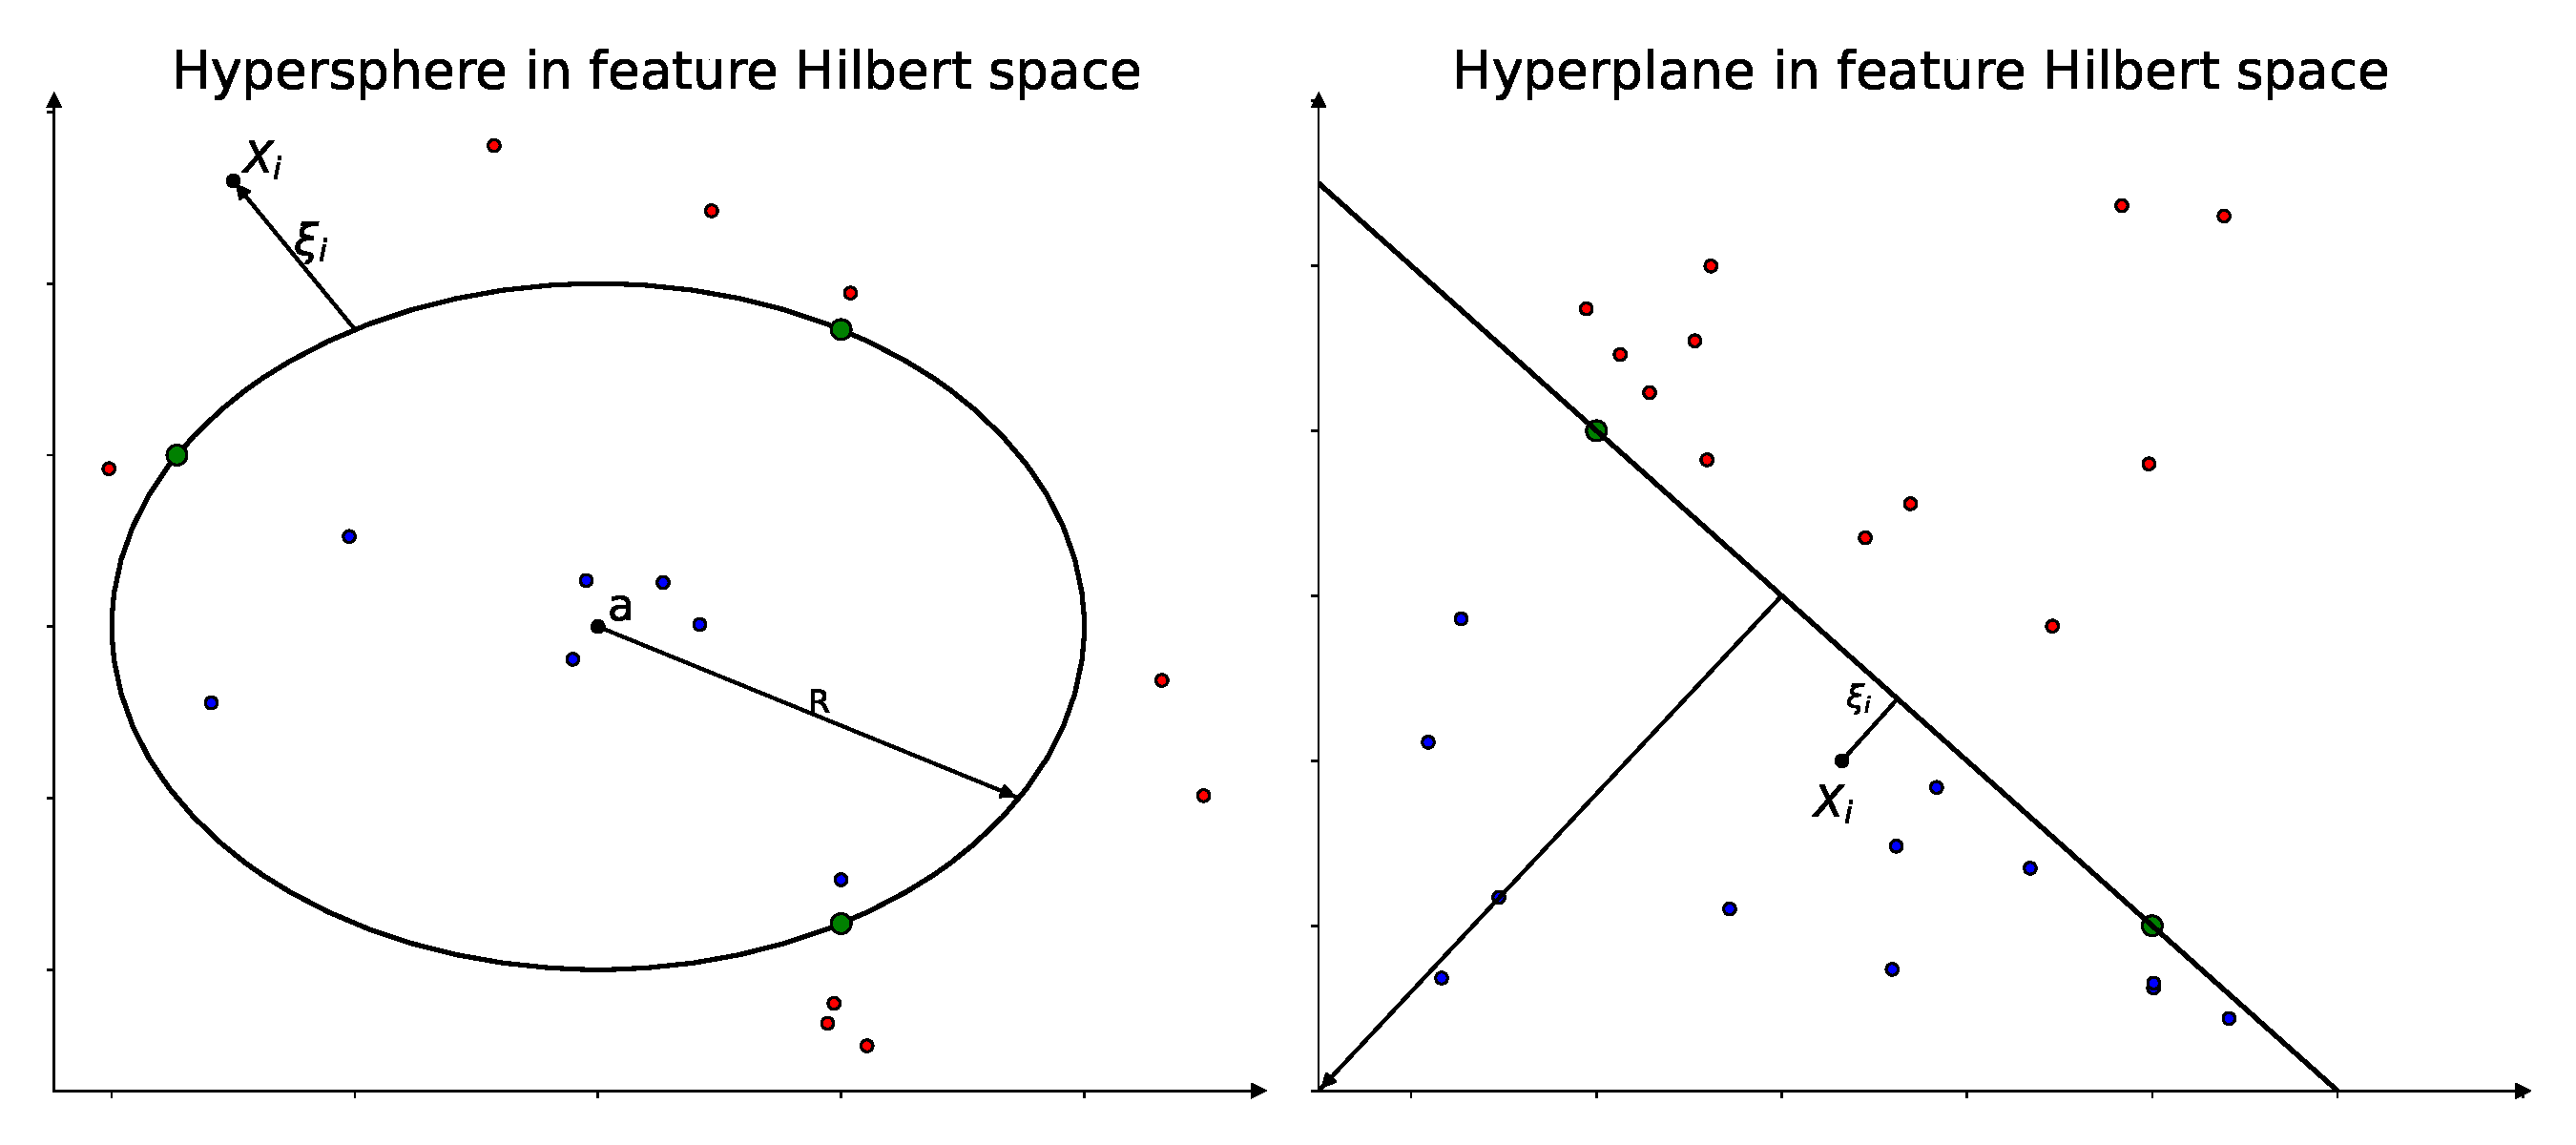
\includegraphics[width=\linewidth]{images/Hyperplane-Hypersphere.pdf}
    \caption{Varianta Schölkopf et al în dreapta şi varianta Tax et al în stânga}
\end{figure}

\section{Caracteristici}

One Class SVM ne ajută să transformăm un model de clasificare 
cu mai multe clase, anume SVM, într-unul cu o singură clasă,
păstrând abilitatea de a putea introduce neliniarități 
cu ajutorul funcţiilor de kernel ce au fost studiate extensiv.
Prin urmare, are majoritatea avantajelor celui din urmă, precum
garanția optimului global datorită funcţiei convexe pe care
o minimizăm, faptul că este relativ robust în spaţii cu 
multe dimensiuni și că poate fi folosit chiar și dacă 
numărul de caracteristici al punctelor din set este mai
mare decât cardinalul setului.

Totuşi, acest model devine imposibil de folosit pentru 
seturi mari de date, complexitatea de timp lasă de dorit 
la antrenare, iar găsirea hiperparametrilor optimi este 
dificilă, atât din lipsa unor reguli stricte după care 
să ne ghidăm, dar și din faptul că o căutare exhaustivă 
ar dura prea mult din cauza complexității de timp ridicate 
la antrenare. De asemenea, rezultatele date de acest model 
nu pot fi ușor interpretate, deoarece ele reprezintă distanțe,
nu probabilități.

\subsection{Formularea matematică}

Prima formulare ce implică un hiperplan de separare

\begin{equation}
    \begin{aligned}
    & \underset{w, \rho, \xi}{\text{min}}
    & & \frac{1}{2} \|w\|^2 + \frac{1}{\nu n} \sum_{i=1}^{n} \xi_i - \rho \\
    & \text{cu constrângerea}
    & & \langle w, \phi(x_i) \rangle \geq \rho - \xi_i, \quad i=1,2,\ldots,n \\
    &&& \xi_i \geq 0, \quad i=1,2,\ldots,n \\
    \end{aligned}
    \end{equation}
    
    \begin{itemize}
        \item $w$ este vectorul de pondere al hiperplanului
        \item $\rho$ este termenul de influenţă
        \item $\xi_i$ sunt variabilele de relaxare pentru încălcarea marginii
        \item $\phi(x_i)$ este funcţia de scufundare pentru $x_i$.
        \item $n$ este numărul total de puncte
        \item $\nu$ este marginea superioară pentru ponderea de anomalii şi marginea 
        inferioară pentru ponderea de vectori suport
    
    \end{itemize}


    împreună cu forma sa duală ce implică folosirea unei funcţii kernel pentru găsirea unui hiperplan 
    de separare într-un spaţiu cu mai multe dimensiuni decât cel iniţial


    \begin{equation}
        \begin{aligned}
        & \underset{\alpha}{\text{min}}
        & & \frac{1}{2} \sum_{i=1}^{n} \sum_{j=1}^{n} \alpha_i \alpha_j K(x_i, x_j) \\
        & \text{cu constrângerea}
        & & 0 \leq \alpha_i \leq \frac{1}{\nu n}, \quad i=1,2,\ldots,n \\
        &&& \sum_{i=1}^{n} \alpha_i = 1
        \end{aligned}
        \end{equation}
    
    \begin{itemize}
        \item $\alpha_i$ sunt variabilele duale asociate punctelor 
        \item $K(x_i, x_j)$ este funcţia kernel
    \end{itemize}

A doua formulare ce implică găsirea hipersferei minime

    \begin{equation}
        \begin{aligned}
        & \underset{R, \rho, \xi}{\text{min}}
        & & R^2 + \frac{1}{\nu n} \sum_{i=1}^{n} \xi_i \\
        & \text{cu constrângerea}
        & & \|\phi(x_i) - c\|^2 \leq R^2 + \xi_i, \quad i=1,2,\ldots,n \\
        &&& \xi_i \geq 0, \quad i=1,2,\ldots,n \\
        \end{aligned}
        \end{equation}
        
        \begin{itemize}
        \item $R$ este raza hipersferei
        \item $c$ este centrul hipersferei
        \end{itemize}
        

\section{Gaussian Mixture Model}

\subsection{Ideea algoritmului}

Este prea restrictiv să presupunem ca fiecare punct dintr-un set de date 
provine din aceeaşi distribuţie unimodală. Prin urmare, a apărut tehnica de bază 
\textbf{"Mixture model"} ce îşi propune să elimine presupunerea anterioară pentru 
a putea modela şi distribuţii multimodale care poate nu provin nici măcar din aceeaşi 
familie, utilizând o sumă ponderată de mai multe componente cu proprietăţi
cunoscute. Totuşi, în practică, se folosesc componente din aceeaşi familie pentru 
modelarea distribuţiei doar că fiecare componentă are parametri diferiţi.

Algoritmul încearcă să estimeze funcţia densitate de probabilitate 
din care au fost generate datele folosind 
\textbf{mai multe distribuţii Gaussiene}.
Astfel, putem modela distribuţii multimodale utilizând o distribuţie bine cunoscută.
Parametrii necesari sunt mediile şi covarianţele fiecărei componente.

\begin{figure}[H]
    \centering
    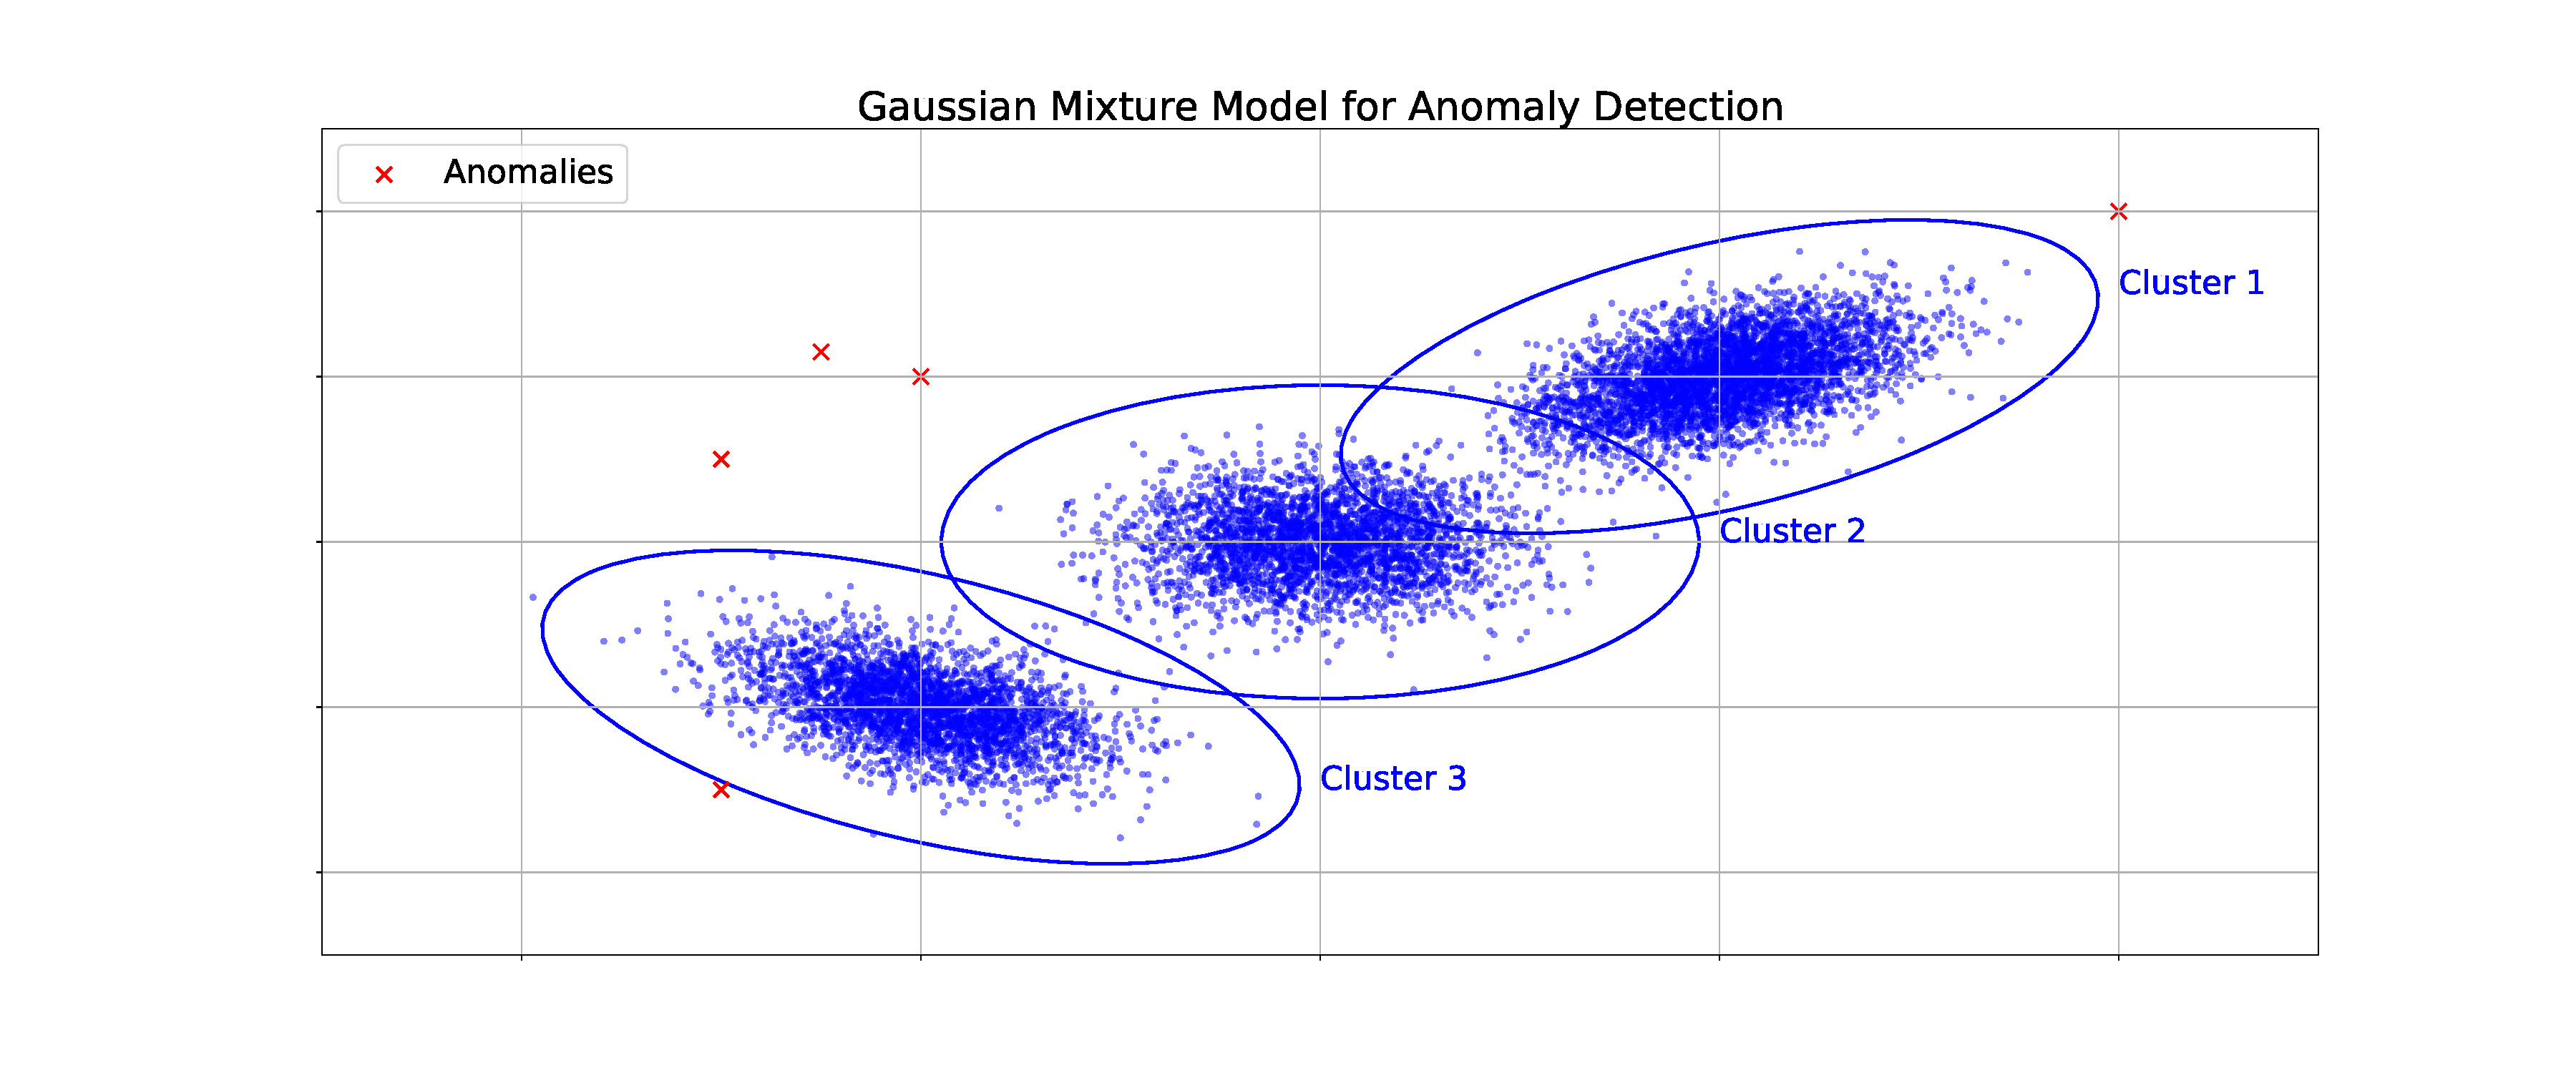
\includegraphics[width=\linewidth]{images/Anomaly-detection-with-Gaussian-mixture-models.pdf}
    \caption{Anomaliile se află în afara distribuţiilor date de componentele Gaussiene}
\end{figure}

\section{Caracteristici}

Gaussian Mixture Model este util pentru modelarea distribuţiilor 
complexe și se descurcă bine chiar și când setul de date 
este compus din mulțimi suprapuse de puncte, întrucât află 
pentru fiecare componentă probabilitatea ca o observaţie
să fie membra acesteia, deci chiar dacă un punct se află 
în mai multe mulțimi, nu va fi repartizat doar în una singură.
De asemenea, timpul de antrenare este redus chiar și pentru 
seturi mari de date datorită tehnicii iterative de optimizare 
utilizată.

Din păcate, numărul de componente nu este ușor de ales 
pentru a obține un model optim, iar performanţa algoritmului 
depinde foarte mult de inițializarea parametrilor iniţiali, 
ceea ce poate duce la imposibilitatea convergenței către optim.
De asemenea, se presupune că datele pot fi modelate de o 
combinație de distribuţii Gaussiane, dar dacă acest lucru 
nu este adevărat, algoritmul nu va oferi rezultate bune.
Un alt dezavantaj este vulnerabilitatea la blestemul 
dimensionalității.

\subsection{Formularea matematică}

Funcţia densitate de probabilitate estimată este dată de 

\begin{equation}
    \text{p}(x) = 1 - \prod_{i=1}^{K} \left(1 - \mathcal{N}(x|\mu_i, \Sigma_i)\right)
\end{equation}
    
\begin{itemize}
    \item $K$ este numărul de componente Gaussiene
    \item $\mathcal{N}(x | \mu_i, \Sigma_i)$ este distribuţia Gaussiană
    cu medie $\mu_i$ şi matrice de covarianţă $\Sigma_i$

Parametrii $\theta$ sunt de obicei învăţaţi din setul de date folosind 
tehnici precum algoritmul Expectation-Maximization (EM).
\end{itemize}

Această formulă ne indică probabilitatea ca un punct să fi fost generat de oricare 
dintre componentele Gaussiene implicate. Deci, o valoare cât mai mică sugerează 
o şansă mare ca punctul să fie anomalie.

\section{Kernel Density Estimation}

\subsection{Ideea algoritmului}

Precum Gaussian Mixture Model, algoritmul încearcă să estimeze 
funcţia densitate de probabilitate din care au fost generate datele.

Tehnica de bază utilizează un kernel funcţie de distribuţie probabilitate
pe care "îl plasăm" la fiecare punct din setul de date, căruia îi oferim o pondere 
de $\frac{1}{n}$, unde $n$ este numărul de observaţii. Apoi, distribuţia adevărată
este aproximată prin adunarea tuturor rezultatelor precedente. Procesul este similar 
aflării ariei de sub graficul unei funcţii cu ajutorul unei integrale ce 
apare dintr-o sumă de valori ale funcţiei într-o infinitate de puncte.

Un parametru numit \textbf{"lăţime de bandă"} influenţează netezimea distribuţiei 
rezultate.
Cel mai des utilizat kernel este cel Gaussian şi pe acesta îl vom folosi şi noi.

Aici, pentru fiecare punct generăm o distribuţie Gaussiană cu \textbf{media} egală
cu punctul respectiv şi \textbf{deviaţie} egală cu "lăţimea de bandă". Apoi, adunăm toate 
distribuţiile obţinute mai sus si le împărţim la numărul total de puncte.

\begin{figure}[H]
    \centering
    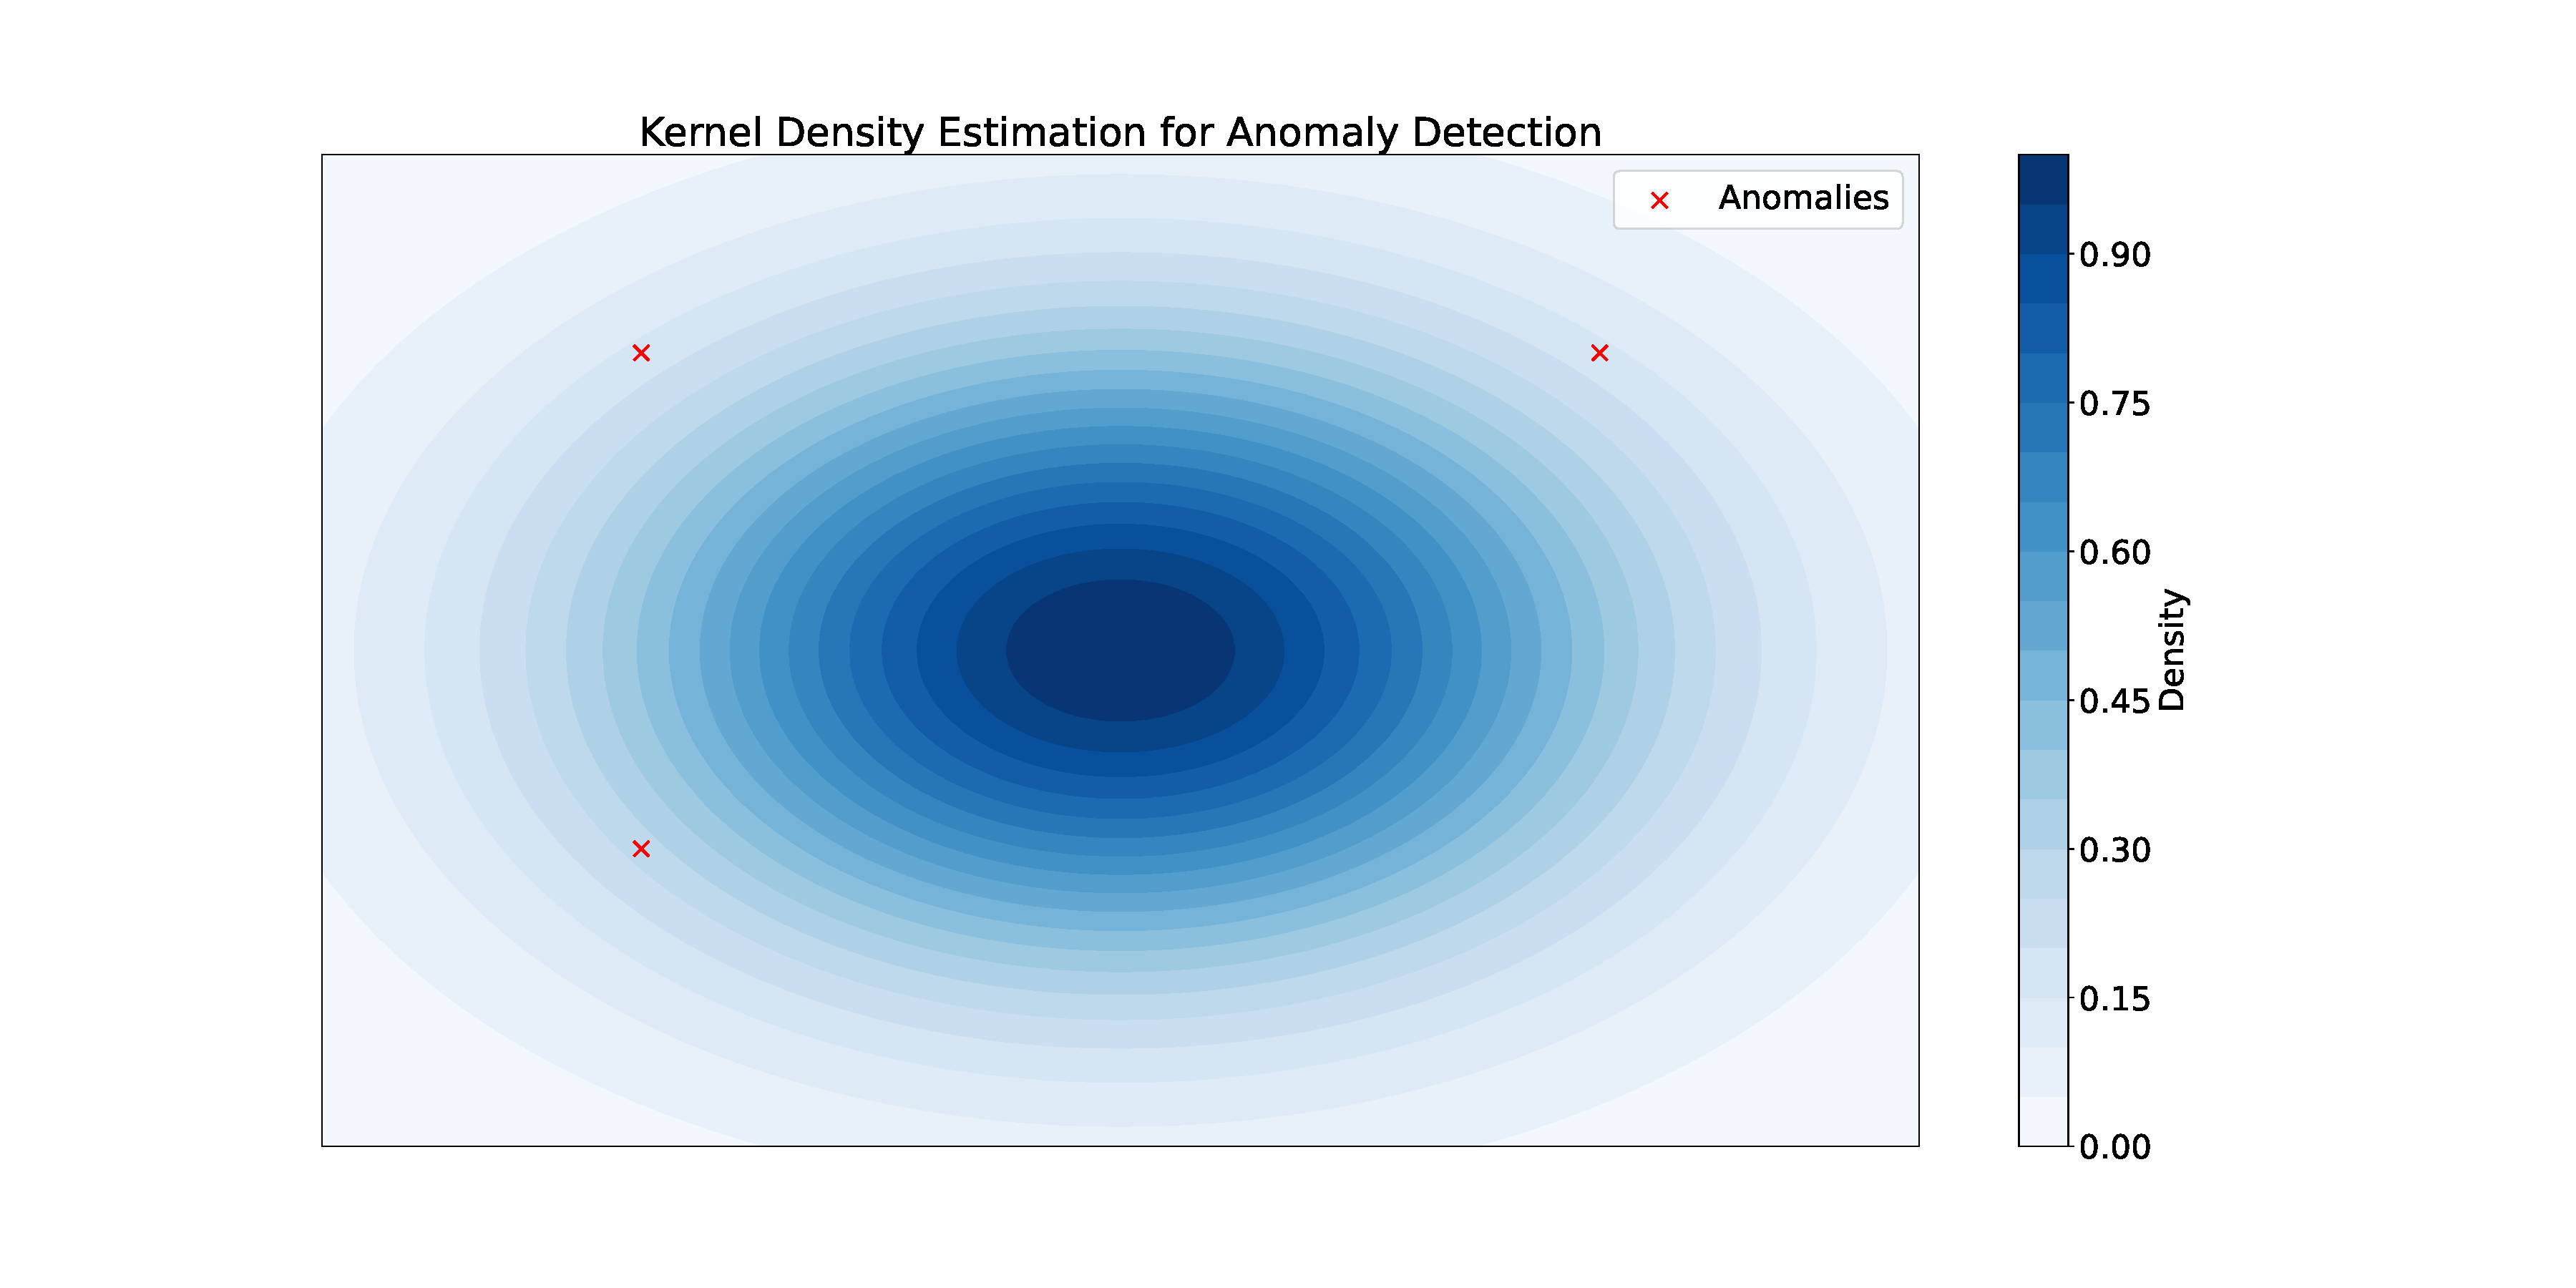
\includegraphics[width=\linewidth]{images/KDEShowOff.pdf}
    \caption{Anomaliile sunt reprezentate de punctele roşii}
\end{figure}

\section{Caracteristici}

Kernel Density Estimation are avantajul de a fi o metoda 
neparametrică și care nu face nicio presupunere asupra 
distribuţiei reale a datelor, ceea ce îl face flexibil 
pentru diverse tipuri de date. De asemenea, rezultatele 
sunt ușor de interpretat acestea fiind probabilități și 
beneficiem de informație locală despre
densitatea datelor în jurul fiecărui punct 
din set, ceea ce ne ajută la găsirea regiunilor cu densitate ridicată 
sau scăzută.

Dezavantajele sunt găsirea dificilă a hiperparametrului 
optim pentru 
lăţime de bandă, complexitatea de timp crescută, în special 
pentru seturi de date mari, vulnerabilitatea la blestemul 
dimensionalității, dar și tendința de a atribui o densitate 
ridicată punctelor din marginea setului de date, chiar 
dacă distribuţia nu se mai întinde în direcția respectivă, 
iar acest lucru poate duce la netezirea excesivă a marginilor 
distribuţiei.

\subsection{Formularea matematică}

Densitatea estimată de kernel într-un punct $x$ este dată de

\begin{equation}
\hat{f}_h(x) = \frac{1}{nh} \sum_{i=1}^{n} K\left(\frac{x - x_i}{h}\right)
\end{equation}

\begin{itemize}
    \item $n$ este numărul total de puncte
    \item $h$ este lăţimea de bandă
    \item $K(u)$ este funcţia kernel 
\end{itemize}

\section{Metrici de performanţă}

Setul de date prezentat în această lucrare este adnotat în întregime, aşa 
că putem folosi aceleaşi tehnici de evaluare a performanţei utilizate pentru
clasificarea binară.

Prin urmare, are sens să folosim următoarele noţiuni ce vor fi utile pentru
descrierea metricilor de performanţă prezentate mai jos:

\begin{itemize}
    \item \textbf{TP} (\textit{true positive}) - reprezintă observaţiile din clasa 
    \textbf{pozitivă} ce au fost clasificate \textbf{corect}
    \item \textbf{TN} (\textit{true negative}) - reprezintă observaţiile din clasa 
    \textbf{negativă} ce au fost clasificate \textbf{corect}
    \item \textbf{FP} (\textit{false positive}) - reprezintă observaţiile din clasa 
    \textbf{pozitivă} ce au fost clasificate \textbf{greşit}
    \item \textbf{FN} (\textit{false negative}) - reprezintă observaţiile din clasa 
    \textbf{negativă} ce au fost clasificate \textbf{greşit}
\end{itemize}
În cazul nostru, clasa \textbf{pozitivă} este reprezentată de \textbf{anomalii}, iar 
clasa \textbf{negativă} este reprezentată de datele \textbf{normale}.

Metricile descrise în această lucrare reprezintă o alegere personală pe care o facem, astfel
încât să reflecte cât mai bine nevoile problemei expuse şi nicidecum nu reprezintă singura
sau cea mai bună cale de a evalua performanţa algoritmilor. Putem pune în paralelă cu teorema
\textbf{"No Free Lunch"} care ne spune că nu există un model care să fie cel mai bun în toate situaţiile,
ci că utilitatea acestuia depinde strict de context. La fel este şi în cazul măsurilor de evaluare,
iar acest fapt face găsirea uneltei potrivite pentru problemă una nu tocmai simplă, ba chiar 
poate necesita un timp considerabil de gândire.

\subsection{Accuracy}

\begin{equation}
    \text{Accuracy} = \frac{TP + TN}{TP + TN + FP + FN}
\end{equation}

Această metrică ne indică câte 
\textbf{clasificări făcute de model au fost corecte din 
totalul de puncte care trebuie clasificate}.

\subsection{Precision}

\begin{equation}
    \text{Precision} = \frac{TP}{TP + FP}
\end{equation}

Precision ne indică \textbf{capacitatea modelului de a nu produce fals pozitive}, în cazul nostru,
de a nu raporta o valoare normală ca fiind anomalie.

\subsection{Recall}

\begin{equation}
    \text{Recall} = \frac{TP}{TP + FN}
\end{equation}

Recall ne indică 
\textbf{capacitatea modelului de a identifica toate observaţiile pozitive},
în cazul nostru, de a detecta toate anomaliile.

\subsection{F1 score}

\begin{equation}
    \text{F1 Score} = \frac{2 \cdot \text{Precision} \cdot \text{Recall}}{\text{Precision} + \text{Recall}}
\end{equation}

F1 score reprezintă \textbf{media armonică dintre precision şi recall}. Prin urmare, f1 score 
va tinde către valoarea mai mică dintre aceste 2 metrici. Pentru a o maximiza,
ar trebui sa avem o valoare mare atât pentru precision, cât şi pentru recall,
fapt ce ar duce la un model ideal.

\subsection{AUC şi ROC Curve}

ROC Curve ne ajută să evaluăm calitatea modelului prin reprezentarea grafică 
a ratei de fals pozitiv pe axa X şi a ratei de adevărat pozitiv pe axa Y. 
\textbf{Punctul 
ideal al graficului se află în colţul din stânga sus} pentru ca ne dorim o 
rată de fals pozitiv egală cu 0 şi o rată de adevărat pozitiv egală cu 1. Prin urmare,
ne dorim sa maximizăm rata de adevărat pozitiv şi de a minimiza rata de fals pozitiv.

Pentru a crea graficul, avem nevoie de \textbf{probabilităţile sau valorile de încredere} 
pentru fiecare observaţie din setul de  testare, generate de funcţia de decizie a 
modelului respectiv. Punctele de pe grafic pot fi văzute precum clasificatoare 
separate ce diferă prin \textbf{pragul} aplicat funcţiei de decizie. Prin urmare, dacă
dorim să ilustrăm ROC Curve, avem nevoie de un algoritm ce are ca valori de ieşire
scoruri care pot fi comparate. One Class SVM, prin definiţie, nu oferă astfel de 
rezultate, aşa că va trebui să îl tratăm în mod diferit.

\textbf{Funcţia de decizie} este cea care atribuie un scor pentru 
un punct din set cu scopul de a indica nivelul de normalitate sau de anomalie 
al acestuia. Generarea etichetei se face apoi folosind un prag în cazul 
probabilităţilor, precum Gaussian Mixture Model şi Kernel Density Estimation, 
sau efectiv reducând valorile pozitive la $+1$ şi pe cele negative la $-1$,
precum One Class SVM.

Totuşi, ROC Curve are caracter vizual şi nu ne oferă o măsură concretă a performanţei.
De aceea, avem nevoie de \textbf{AUC}, valoare ce reprezintă aria de sub grafic. Cu cât aria
este mai mare, cu atât modelul este mai bun.

\subsection{Micro average vs Macro average}

Nu există o singură metodă de evaluare a modelelor care să fie potrivită în toate 
cazurile. În schimb, metodele sunt alese astfel încât să reflecte cât mai bine 
nevoile problemei.

\textbf{Macro} average pentru o măsură de evaluare are forma:

$$B_{macro}=\frac{1}{q} \sum_{\lambda=1}^{q} B(tp_{\lambda}, tn_{\lambda}, fp_{\lambda},
fn_{\lambda})$$

\textbf{Micro} average pentru o măsură de evaluare are forma:

$$B_{micro}=B(\sum_{\lambda=1}^{q} tp_{\lambda}, \sum_{\lambda=1}^{q} tn_{\lambda}, 
\sum_{\lambda=1}^{q} fp_{\lambda}, \sum_{\lambda=1}^{q} fn_{\lambda})$$

$L=\{\lambda_{j}: j=1,\dots,q \}$ este setul tuturor etichetelor asociate claselor, iar 
$B(tp, tn, fp, fn)$ este o măsură de evaluare binară bazată pe noţiunile introduse mai sus
\cite{Asch2013MacroandME}.
În cazul nostru, $\lambda=2$.


Diferenţa între cele 2 metode este că macro average acordă o importanţă 
\textbf{egală fiecărei 
clase}, pe când micro average acordă o importanţă 
\textbf{egală fiecărei observaţii}. Prin urmare,
varianta micro favorizează clasa 
\textbf{majoritară} la calcularea scorului, în timp ce varianta 
macro favorizează clasa \textbf{minoritară}.

Ilustrăm aceste diferenţe printr-un exemplu ce are ca măsură de evaluare binară 
\textbf{accuracy},
şi care arată cum metodele acoperă nevoi diferite.

Ponderea claselor este extrem de neechilibrată în setul nostru de date, anomaliile 
reprezentând doar $0.017\%$ din total. Prin urmare, dacă dorim să maximizăm 
micro average accuracy, putem alege un model trivial ce mereu prezice clasa majoritară.
Am obţine un accuracy de peste $99.9\%$ cu un minim de efort!

Este impresionant, dar modelul de mai sus este practic inutil pentru problema noastră.
Toate anomaliile ar trece nedetectate. În schimb, dacă am evalua acelaşi model folosind
varianta macro average, am obţine un accuracy de doar $50\%$. Modelul este acum inutil,
întrucât suntem interesaţi să detectăm anomaliile, nu doar să punem eticheta corectă 
pe cât mai multe observaţii indiferent de clasă.

Astfel, vom folosi varianta macro average pentru accuracy, iar pentru precision, recall şi 
f1 score, vom calcula rezultatul folosind clasa minoritară ca referinţă. Decizia este influenţată
de faptul că vrem să urmărim performanţa modelului pe detectarea anomaliilor în special, cu ajutorul
precision şi recall, dar în acelaşi timp vrem să obţinem un echilibru între fals pozitive şi 
adevărat pozitive, utilizând accuracy împreună cu f1 score, metode ce iau în calcul performanţa 
per total pe ambele clase. Este important să detectăm cât mai multe fraude, dar în acelaşi timp 
nu ne dorim să semnalăm un număr prea mare de tranzacţii ca fiind problematice deoarece modelul 
ar deveni un inconvenient.
\chapter{Explorarea setului de date}

\section{Descriere}

Acest set de date conţine informaţii despre 284,807 de tranzacţii dintre care 
492 sunt \textbf{frauduloase}. Conţine doar variabile numerice.

Din motive de confidenţialitate, dimensiunea trăsăturilor originale a fost 
redusă folosind \textbf{Analiza Componentelor Principale} (PCA) la 28 de trăsături denumite 
"V1-V28" şi încă 2 trăsături ce nu au fost transformate, anume suma de bani
a tranzacţiei şi timpul relativ, începând de la 0, când aceasta a fost făcută. 
De asemenea, pentru fiecare tranzacţie avem eticheta 0 sau 1, daca este normală 
sau, respectiv, frauduloasă.

\section{Matricea de corelaţie}

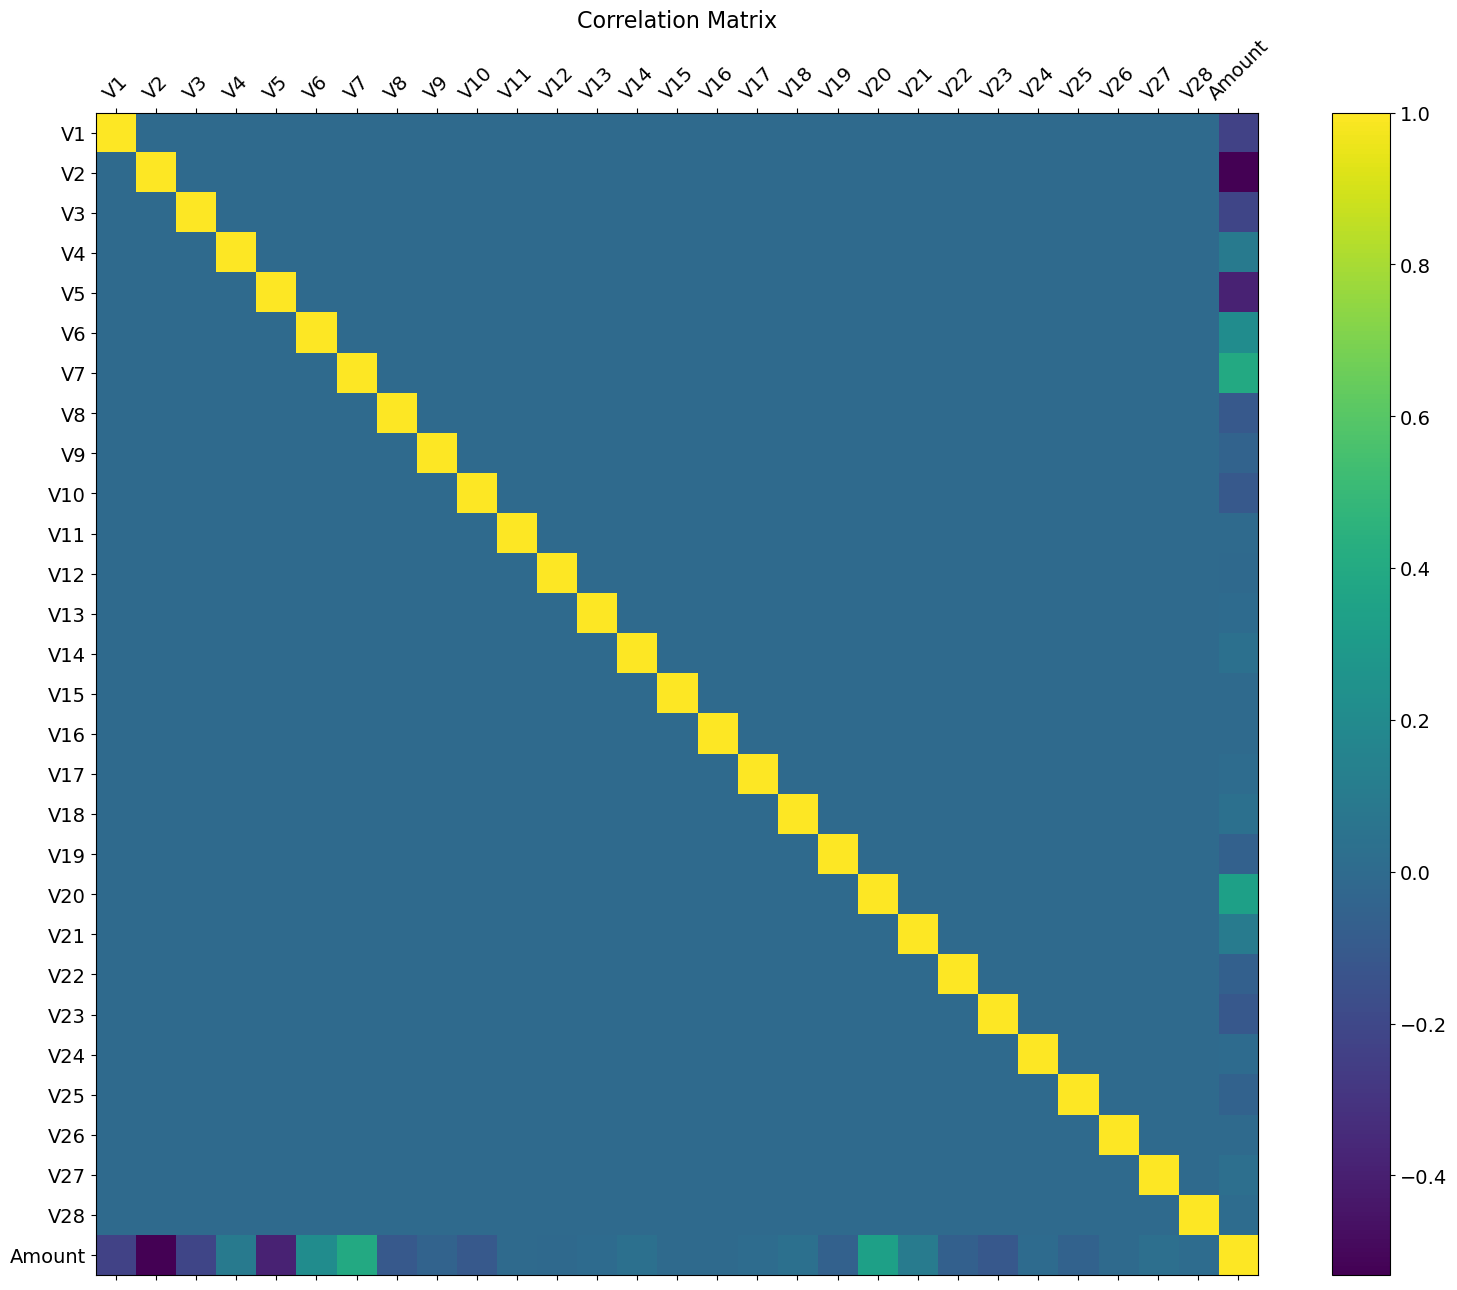
\includegraphics[width=\linewidth]{correlation-matrix.png}

Se observă lipsa corelaţiei între variabilele anonime. Este de aşteptat, totuşi, 
având în vedere că variabilele au fost obţinute prin PCA, care din definiţie generează 
componente \textbf{necorelate liniar}.

Singura corelaţie apare între variabila "Amount" şi restul variabilelor. Corelaţiile
cu o magnitudine semnificativă apar între amount şi V6, V7, V20, cu valoare pozitivă, 
şi între amount şi V1, V2, V5, cu valoare negativă.

\section{Preprocesarea datelor}

\subsection{Eliminăm trăsăturile inutile}

În viaţa reală, data şi ora tranzacţiei ne pot ajuta să depistăm un comportament 
ciudat. Totuşi, aceste informaţii sunt relevante numai atunci când am monitorizat
pe o perioada de măcar câteva zile activitatea din contul/cardul respectiv pentru a 
stabili ce reprezintă un comportament "normal".

În cazul nostru, nu avem la dispoziţie nici măcar data şi ora exactă. Prin urmare, vom
elimina timpul din fiecare observaţie.

De asemenea, eliminăm etichetele. Acestea sunt utile numai la testare pentru a analiza 
performanţa şi la alegerea setului de antrenare. Metodele utilizate în această lucrare
sunt exclusiv \textbf{nesupervizate}, deci nu avem nevoie de etichete la procesul de antrenare.

\subsection{Validarea încrucişată}

Împărţim setul de date în antrenare, validare şi testare cu proporţiile 75\%, 0.15\%
şi, respectiv, 0.10\%. De asemenea, ne asigurăm că 
\textbf{proporţiile de normal/anomalie} 
rămân aproximativ la fel în toate seturile.

Totuşi, pentru că algoritmii prezentaţi "învaţă" structura datelor normale şi avem 
la dispoziţie etichetele, vom elimina din \textbf{setul de antrenare}
toate punctele cu eticheta 
1 şi le vom muta în setul de validare.

\textbf{Setul de validare} va fi folosit pentru alegerea hiperparametrilor optimi, în timp ce 
\textbf{setul de testare} va fi folosit la final pentru a face o comparaţie imparţială 
a performanţei modelelor.

\subsection{Scalare}

Având în vedere că nu cunoaştem mai nimic despre trăsăturile punctelor, vom scala 
datele folosind metoda clasică de 
\textbf{a scădea media şi a împărţi la deviaţia standard}.
Media şi deviaţia standard sunt obţinute din setul de antrenare. Le folosim pe acestea 
să transformăm setul de validare, cât şi pe cel de testare.
\chapter{Evaluarea modelelor}


Căutarea \textbf{hiperparametrilor optimi} se va realiza pentru fiecare model 
în parte folosind setul de validare. La final, cele mai bune modele 
găsite sunt evaluate într-un mod imparţial pe setul de testare. 

\section{Modele nesupervizate}

\subsection{One Class SVM}

Pentru a exploata capabilităţile de modelare a unei margini de decizie 
neliniare a SVM-urilor, avem nevoie de funcţii kernel care să scufunde
punctele din setul de date într-un spaţiu cu mai multe dimensiuni unde 
să putem găsi mai uşor un hiperplan de separare.

\begin{itemize}
    \item \(K(x, y) = x^T y\) - \textbf{Liniar}
    \item \(K(x, y) = (\gamma x^T y + c)^d\) - \textbf{Polinomial}
    \item \(K(x, y) = \exp\left(-\gamma{\|x - y\|^2}\right)\) - \textbf{Gaussian}
    \item \(K(x, y) = \tanh(\gamma x^T y + c)\) - \textbf{Sigmoid}
\end{itemize}

Un caz particular este kernel-ul \textbf{liniar} care păstrează punctele
în spaţiul iniţial şi încearcă să găsească un hiperplan de separare 
optim la fel ca în cazul clasic fără kernel al SVM-ului.
Acest kernel este nepotrivit în cele mai multe cazuri, mai puţin când 
datele sunt aproape liniar separabile, deci nu ne aşteptăm să performeze
excepţional.

Totuşi, putem exploata eficienţa kernel-ului liniar folosind tehnica de 
optimizare \textbf{Stochastic Gradient Descent} (SGD) împreună cu metoda de aproximare 
\textbf{Nystroem} pentru a aplica o transformare neliniară asupra
datelor de intrare şi apoi să găsim o margine de decizie liniară în noul spaţiu.

SGD este o metodă iterativă relativ simplă ce nu necesită un număr la fel de 
mare de calcule şi nici la fel de multă memorie precum metodele clasice 
de rezolvare a unui sistem de ecuaţii folosind algebră liniară. De aceea, este
potrivită atunci când mărimea setului de date trece de ordinul sutelor de mii,
în ciuda faptului că sacrificăm acurateţea ponderilor estimate.

Metoda Nystroem aproximează matricea kernel pentru o anumită funcţie kernel dată,
folosind tehnica aproximării cu \textbf{matrice de 
rang scăzut} unde o fracţiune din punctele setului de antrenare este folosită 
ca bază vectorială pentru kernelul respectiv. Evident, calculul va fi mult mai 
rapid folosind o matrice de dimensiune redusă. Am comparat performanţa acestei metode 
pentru diverse funcţii kernel şi pentru diverse fracţiuni de puncte din setul de 
antrenare, care erau folosite de algoritm. Numărul de puncte a fost selectat astfel 
încât să ocupe un procent, dat ca parametru, din memoria RAM. Prin urmare, rezultatele 
pot să difere în funcţie de capacitatea memoriei pe care o avem la dispoziţie.

Pentru comparaţie am inclus şi funcţiile \textbf{polinomială} şi 
\textbf{sigmoidă}. Cu cea din urmă am obţinut rezultatele cele mai bune în comparaţie
cu celelalte funcţii, dar  
nu mai bune decât kernelul Gaussian pe care îl vom folosi şi care 
este şi decizia des întâlnită în practică. De asemenea, atât kernel-ul liniar pentru valori mai mari
ale lui $\nu$, 
cât şi cel polinomial începând cu gradul 7 nu terminau antrenarea nici măcar 
după 12 ore, aşa că am abandonat căutarea hiperparametrilor pentru mai mult 
de atât, mai ales că acurateţea prezicerilor devenea din ce în ce mai îndoielnică.

\begin{table}[H]
    \centering
    \begin{tabularx}{\textwidth}{
        |X
        |X
        |X
        |X
        |X
        |X
        |X
        |X|
    }
    \hline
    $d$ & $\gamma$ & $\nu$ & {Accuracy} & {Recall} & {Precision} & {F1 Score} \\
    \hline
    \rowcolor{gray!20} 7 & 0.001 & 0.007 & 0.474	& 0.947 & 0.006	& 0.0129    \\
    5 & 0.001 & 0.02 & 0.469	& 0.930	& 0.006	& 0.0128 \\
    \rowcolor{gray!20} 7 & 1 & 0.0001	& 0.502	& 0.0243	& 0.008	& 0.0124   \\
    7 & 2 & 0.0001 & 0.502	& 0.024	& 0.008	& 0.0124 \\
    \hline
  \end{tabularx}
  \caption{Cele mai bune rezultate, în funcţie de F1, obţinute pentru kernel-ul polinomial}
\end{table}

\begin{table}[H]
    \centering
    \begin{tabularx}{\textwidth}{
        |X
        |X
        |X
        |X
        |X
        |X
        |X|
    }
    \hline
    $\gamma$ & $\nu$ & {Accuracy} & {Recall} & {Precision} & {F1 Score} \\
    \hline
    \rowcolor{gray!20} 0.03	& 0.005	& 0.804 & 0.613	& 0.476 & 0.536\\
    0.02 & 0.005 & 0.792 & 0.589 & 0.448 & 0.509 \\
    \rowcolor{gray!20} 0.03	& 0.001	& 0.668 & 0.337	& 0.674 & 0.449    \\
    0.02 & 0.007 & 0.756 & 0.520 & 0.347 & 0.416 \\
    \hline
  \end{tabularx}
  \caption{Cele mai bune rezultate, în funcţie de F1, obţinute pentru kernel-ul sigmoid}
\end{table}

\begin{table}[H]
    \centering
    \begin{tabularx}{\textwidth}{
        |X
        |X
        |X
        |X
        |X
        |X
        |X|
    }
    \hline
    $\nu$ & {Accuracy} & {Recall} & {Precision} & {F1 Score} \\
    \hline
    \rowcolor{gray!20} 0.9 & 0.177 & 0.300 & 0.002 & 0.004    \\
    0.001 & 0.412	& 0.0813	& 0.002	& 0.004 \\
    \hline
  \end{tabularx}
  \caption{Cele mai bune rezultate, în funcţie de F1, obţinute pentru kernel-ul liniar}
\end{table}

\begin{table}[H]
    \centering
    \begin{tabularx}{\textwidth}{
        |X
        |X
        |X
        |X
        |X
        |X
        |X|
    }
    \hline
    $\gamma$ & {Componente} & {Accuracy} & {Recall} & {Precision} & {F1 Score} \\
    \hline
     0.5 & 24394 & 0.752 & 0.979 & 0.0140	& 0.0277 \\
    \rowcolor{gray!20} 0.5	& 22128	& 0.752 & 0.979	& 0.0140 & 0.0277 \\
    0.5	& 11005	& 0.749	& 0.979	& 0.0139 & 0.0274 \\
    \hline
  \end{tabularx}
  \caption{Cele mai bune rezultate, în funcţie de F1, obţinute pentru kernel-ul Gaussian cu SGD şi Nystroem}
\end{table}

\begin{table}[H]
    \centering
    \begin{tabularx}{\textwidth}{
        |X
        |X
        |X
        |X
        |X
        |X
        |X
        |X|
    }
    \hline
    $d$ & $\gamma$ & {Componente} & {Accuracy} & {Recall} & {Precision} & {F1 Score} \\
    \hline
    1 & 1 & 24248 & 0.730 & 0.898 & 0.014 & 0.0275 \\
    \rowcolor{gray!20} 1 &  1 & 5547 & 0.734	& 0.914	& 0.014	& 0.0275 \\ 
    1 & 1 & 16527 & 0.727 & 0.930 & 0.013 & 0.0263 \\ 
    \hline
  \end{tabularx}
  \caption{Cele mai bune rezultate, în funcţie de F1, obţinute pentru kernel-ul polinomial cu SGD şi Nystroem}
\end{table}

\begin{table}[H]
    \centering
    \begin{tabularx}{\textwidth}{
        |X
        |X
        |X
        |X
        |X
        |X
        |X|
    }
    \hline
    $\gamma$ & {Componente} & {Accuracy} & {Recall} & {Precision} & {F1 Score} \\
    \hline
     0.001 & 426 & 0.833 & 0.747 & 0.059 & 0.1108 \\
     \rowcolor{gray!20} 0.001 & 213 & 0.889 & 0.922 & 0.042	& 0.0817 \\
    0.001 & 852	& 0.596 & 0.313 & 0.017	& 0.0337 \\
    \hline
  \end{tabularx}
  \caption{Cele mai bune rezultate, în funcţie de F1, obţinute pentru kernel-ul sigmoid cu SGD şi Nystroem}
\end{table}

Utilizăm kernelul Gaussian, deci printre hiperparametrii optimi pe care îi căutăm 
se va regăsi şi $\gamma$. Acest parametru influenţează 
\textbf{aria zonei de influenţă a 
fiecărui vector suport}. O valoare prea mare ar cauza ca zona să includă numai 
vectorul suport şi nimic altceva, ceea ce ar duce la o \textbf{varianţă crescută} 
a modelului. La polul opus, o valoare prea mică ar cauza ca zona sa includă 
toate punctele din setul de date, ceea ce ar duce la un \textbf{bias crescut}.

Parametrul $\nu$ este similar parametrului $C$ din \textbf{Soft-Margin SVM}, 
cel din urmă
fiind creat cu scopul de a rezolva problemele asociate parametrului $C$, anume că 
putea lua orice valoare pozitivă şi nu avea o interpretare directă. $\nu$ se află 
în intervalul $\left(0, 1\right]$ şi este interpretat ca marginea superioară a ponderii de anomalii 
şi marginea inferioară a ponderii de vectori suport. Prin urmare, $\nu$ controlează
mărimea \textbf{frontierei din jurul datelor normale} a modelului, 
unde o frontieră mai mică este asociată
cu o varianţă crescută, în timp ce o frontiera mai mare este asociată cu un bias 
crescut.

Folosim metoda \textbf{Grid Search} pentru a găsi parametrii favorabili. Afişăm 
doar valorile parametrilor pentru care obţinem rezultate semnificative.

\begin{table}[H]
  \centering
  \begin{tabularx}{\textwidth}{
      |X
      |X
      |X
      |X
      |X
      |X|
  }
  \hline
  $\gamma$ & $\nu$ & {Accuracy} & {Recall} & {Precision} & {F1 Score} \\
  \hline
  \rowcolor{gray!20} 0.01 &  0.0001	&  0.822 &  0.646	&  0.676	&  0.661  \\
  0.01	&  0.001 &  0.822	&  0.646	&  0.676	&  0.661 \\
  \rowcolor{gray!20} 0.01 & 0.005 &  0.875 &  0.756	&  0.531	&  0.624  \\
  0.02 & 0.0001	& 0.877 &  0.760 &  0.526	&  0.622 \\
  \rowcolor{gray!20} 0.02 &  0.001	&  0.877 & 0.760 &  0.523	&  0.620 \\
  \hline
  \end{tabularx}
  \caption{Cele mai bune rezultate, în funcţie de F1, obţinute pentru kernel-ul Gaussian}
\end{table}

Se observă că $\gamma$ este parametrul care aduce schimbările drastice în valorile 
metricilor, pe când $\nu$ doar creşte sau scade relativ puţin aceste valori.

Urmărim F1 score, aceasta fiind metrica ce evaluează modelul oarecum 
echilibrat, în contrast cu precision şi recall care favorează minimizarea fals pozitivelor, 
respectiv a fals negativelor. Astfel, alegem $\gamma=0.01$ şi $\nu=0.0001$ pentru modelul final.

\begin{figure}[!htb] % Use a separate page for the figure
    \begin{minipage}[t]{0.5\textwidth}
        \vspace{0pt}
        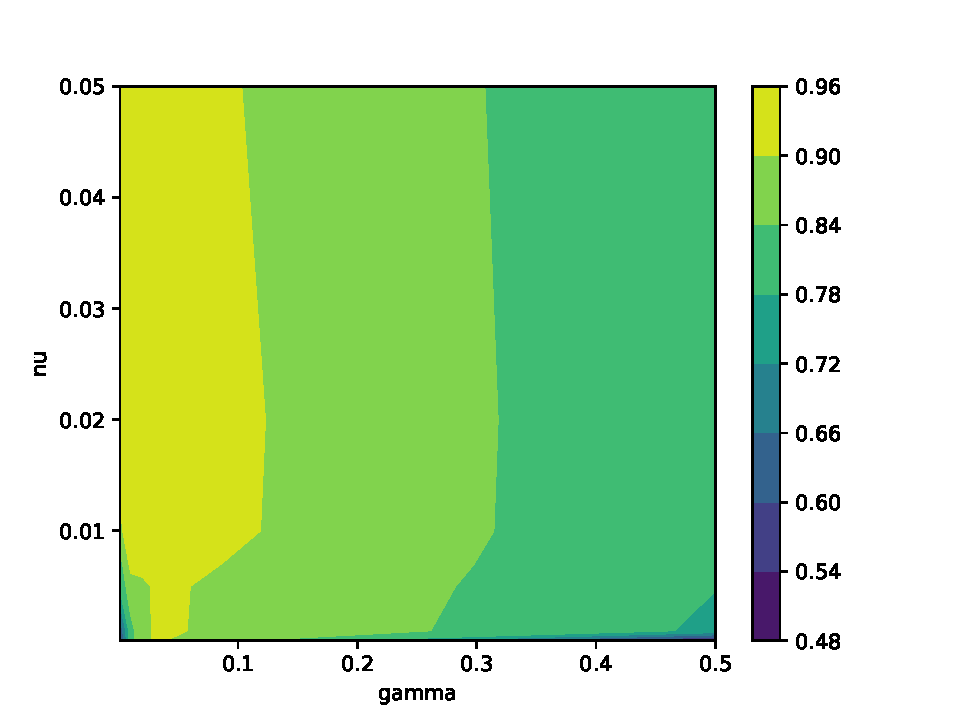
\includegraphics[width=\textwidth]{images/ocsvm-accuracy.pdf}
        \caption{OCSVM Accuracy}
    \end{minipage}
    \hfill
    \begin{minipage}[t]{0.5\textwidth}
        \vspace{0pt}
        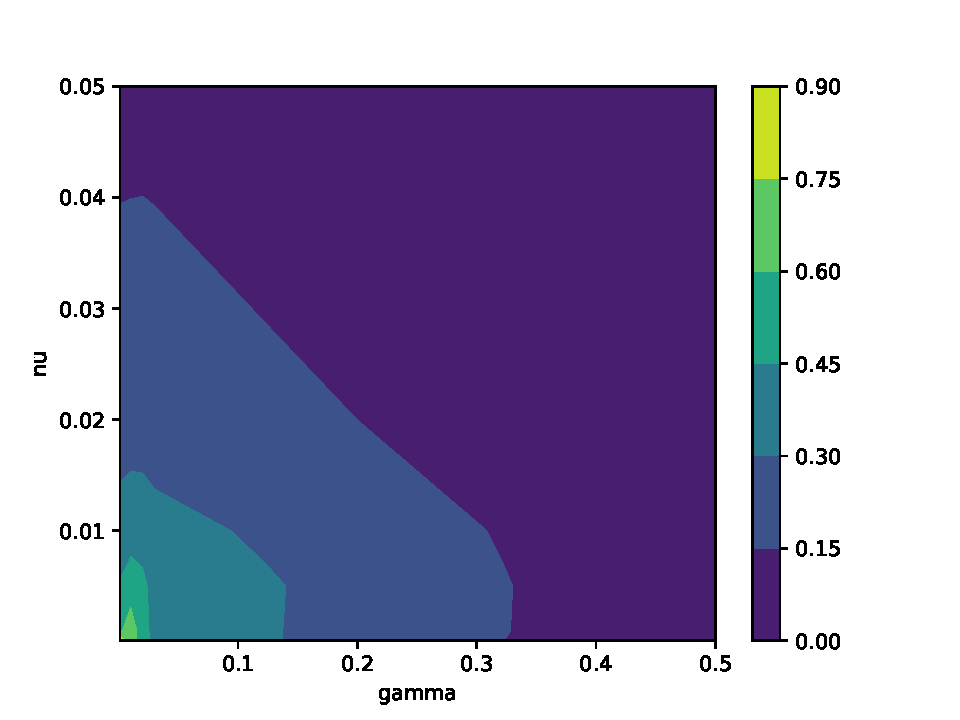
\includegraphics[width=\textwidth]{images/ocsvm-precision.pdf}
        \caption{OCSVM Precision}
    \end{minipage}
    \\
    \begin{minipage}[t]{0.5\textwidth}
        \vspace{0pt}
        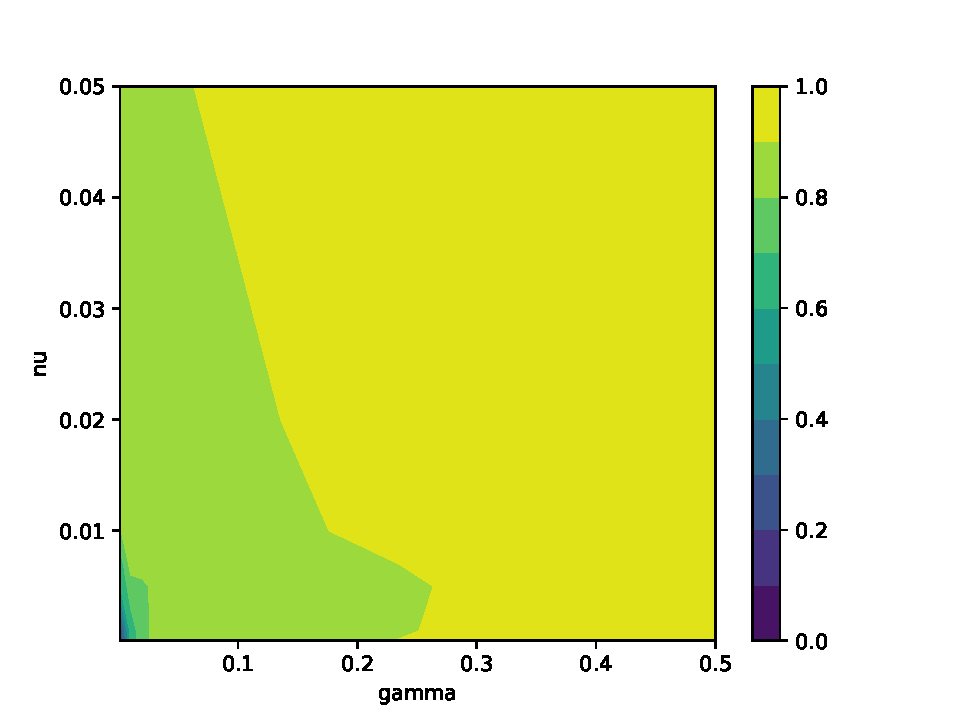
\includegraphics[width=\textwidth]{images/ocsvm-recall.pdf}
        \caption{OCSVM Recall}
    \end{minipage}
    \hfill
    \begin{minipage}[t]{0.5\textwidth}
        \vspace{0pt}
        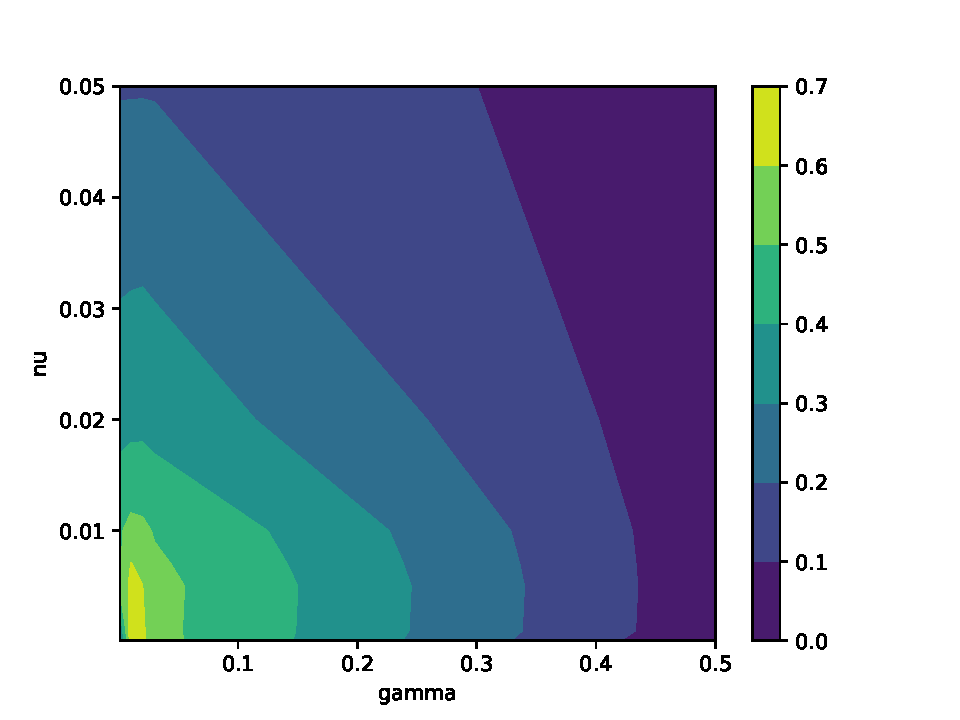
\includegraphics[width=\textwidth]{images/ocsvm-f1.pdf}
        \caption{OCSVM F1 score}
    \end{minipage}
\end{figure}

\noindent

\subsection{Gaussian Mixture Model}

\begin{table}[H]
  \centering
  \begin{tabularx}{\textwidth}{
      |X
      |X
      |X
      |X
      |X
      |X|
  }
  \hline
  $K$ & $q$ & {Accuracy} & {Recall} & {Precision} & {F1 Score} \\
  \hline
  \rowcolor{gray!20} 4 & 0.01 & 0.920 & 0.845 & 0.581 & 0.688  \\
  3	& 0.01 & 0.918	& 0.841 & 0.578 & 0.685 \\
  \rowcolor{gray!20} 2	& 0.01 & 0.918 & 0.841 & 0.578	& 0.685  \\
  1 & 0.01 & 0.914 & 0.833 & 0.572 & 0.678 \\
  \rowcolor{gray!20} 5 & 0.01 & 0.912	& 0.829 & 0.569	& 0.675  \\
  \hline
  \end{tabularx}
  \caption{Cele mai bune rezultate, în funcţie de F1, obţinute pentru Gaussian Mixture Model}
\end{table}



Pentru acest model, hiperparametrul optim 
căutat este numărul de componente Gaussiene $K$. Vom încerca pe rând fiecare valoare
din $K\in\{1, 2, 3, \ldots, 16, 17\}$. De asemenea, pentru că modelul 
ne va oferi probabilitățile de apartenență a unui punct pentru 
fiecare componentă, vom avea nevoie și de un prag pentru a decide 
dacă punctul este sau nu anomalie. Ne vom folosi de cuantile 
calculate pe setul de validare pentru a găsi pragul optim.

Pentru $K=1$ putem afla parametrii foarte eficient folosind 
\textbf{Maximum Likelihood Estimation}, întrucât problema 
se reduce la aflarea mediei şi a matricei de 
covarianţă pentru o distribuţie Gaussiană. 

Pentru $K > 1$ vom folosi \textbf{Expectation Maximization} 
pentru a găsi parametrii optimi, 
având în vedere ca numărul de componente este precizat de la început.

Gaussian Mixture Model încearcă să estimeze o distribuţie posibil multimodală 
folosind mai multe componente Gaussiene. Prin urmare, numărul optim de componente
ne indică intuitiv numărul de \textbf{moduri} pe care le are distribuţia ce a generat 
setul de date.
Se observă că modelul se descurcă destul de bine chiar şi cu o singură componentă. 
Aceasta ne indică faptul ca distribuţia ce a generat setul de date este 
similară cu una Gaussiană.

Pentru acest model, pragul este foarte important. Dacă avem acelaşi prag,
dar număr de componente diferite, varianţa rezultatelor
nu este prea mare, dar dacă alegem greșit valoarea cuantilei, 
performanţa modelului are de suferit. Totuşi, 
dată simplitatea modelului, rezultatele sunt impresionante.
Cu un timp de antrenare de sub câteva minute, obține rezultate 
mai bune decât One Class SVM pe setul de validare.

Alegem \textbf{numărul de componente $K=4$} şi valoarea
cuantilei $q=0.01$ pentru modelul final, chiar dacă 
am avut rezultate bune şi cu $K=1$ deoarece ne dorim un model puţin mai complex 
decât o banală distribuţie Gaussiană. În practică, este o şansă mică să dăm peste 
un proces care să genereze date fix în acest mod. De asemenea, aici F1 score are valoarea cea mai mare
şi după aceasta ne vom ghida, având în vedere că ne interesează performanţa modelului 
per total.

\begin{figure}[!htb] % Use a separate page for the figure
    \begin{minipage}[t]{0.5\textwidth}
        \vspace{0pt}
        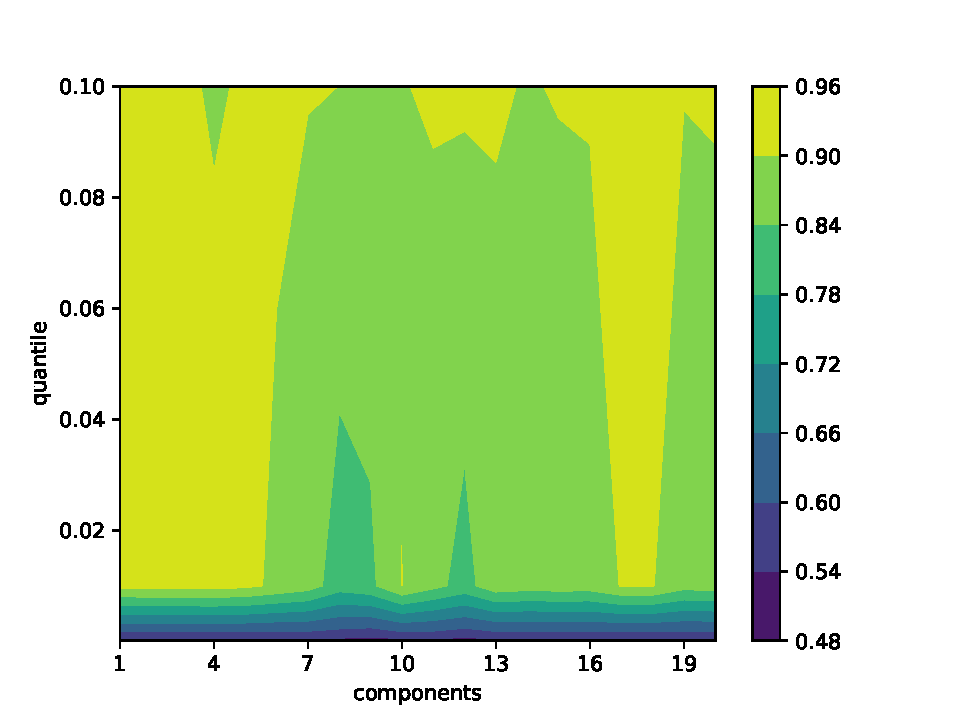
\includegraphics[width=\textwidth]{images/gmm-accuracy.pdf}
        \caption{GMM Accuracy}
    \end{minipage}
    \hfill
    \begin{minipage}[t]{0.5\textwidth}
        \vspace{0pt}
        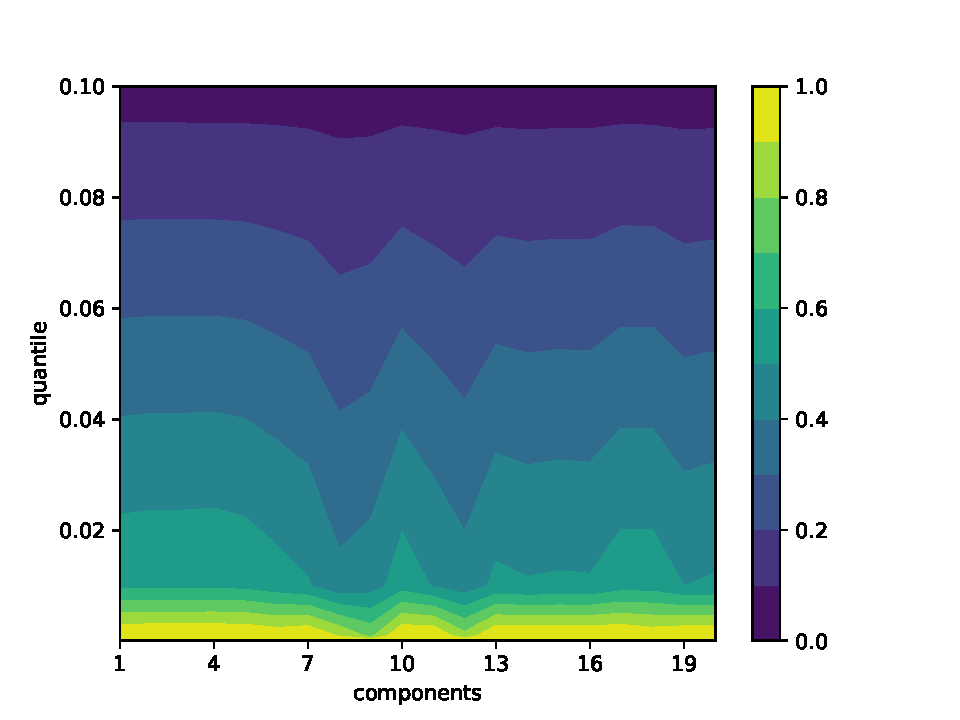
\includegraphics[width=\textwidth]{images/gmm-precision.pdf}
        \caption{GMM Precision}
    \end{minipage}
    \\
    \begin{minipage}[t]{0.5\textwidth}
        \vspace{0pt}
        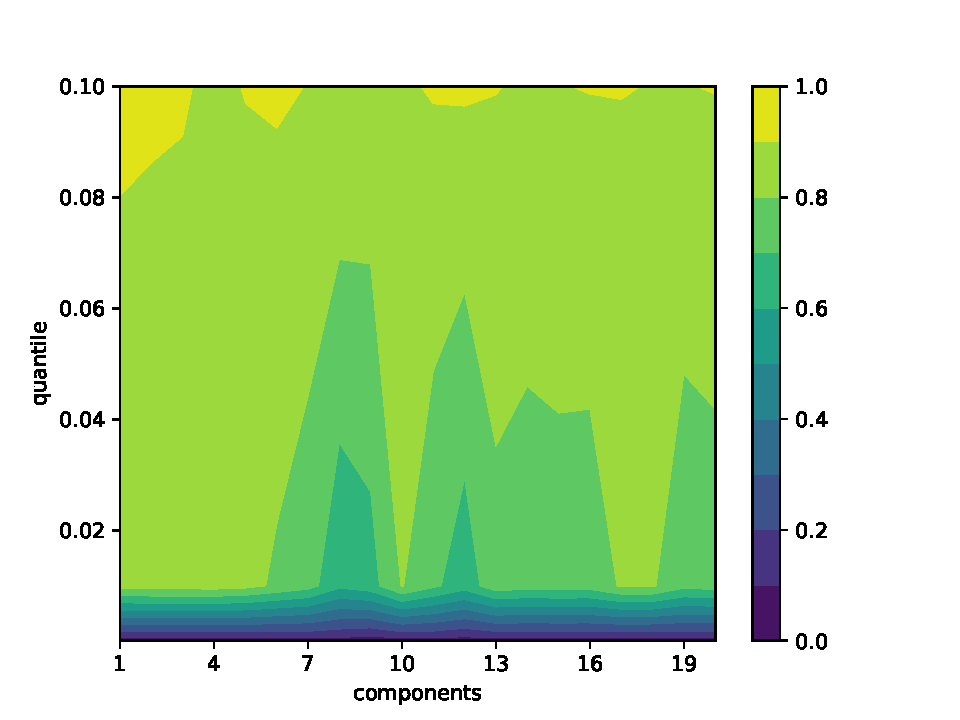
\includegraphics[width=\textwidth]{images/gmm-recall.pdf}
        \caption{GMM Recall}
    \end{minipage}
    \hfill
    \begin{minipage}[t]{0.5\textwidth}
        \vspace{0pt}
        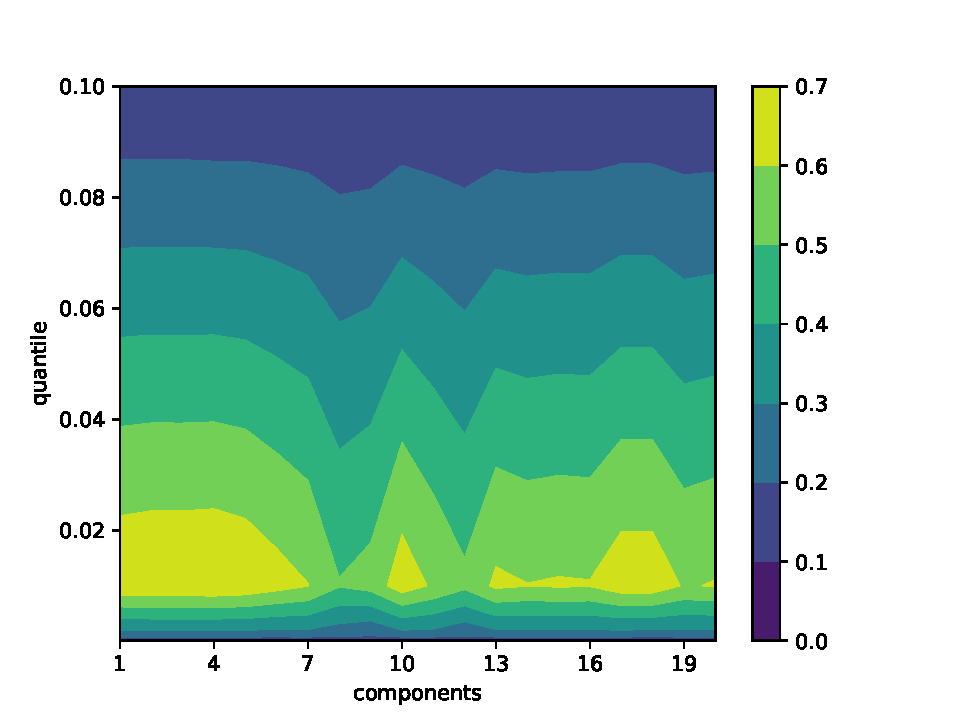
\includegraphics[width=\textwidth]{images/gmm-f1.pdf}
        \caption{GMM F1 score}
    \end{minipage}
\end{figure}

\noindent
  

\subsection{Kernel Density Estimation}

\begin{table}[H]
  \centering
  \begin{tabularx}{\textwidth}{
      |X
      |X
      |X
      |X
      |X
      |X
      |X
      |X|
  }
  \hline
  $Kernel$ & $h$ & $q$ & {Accuracy} & {Recall} & {Precision} & {F1 Score} \\
  \hline
  \rowcolor{gray!20} tophat	& 9	& 0.01 & 0.908 & 0.821 & 0.562 & 0.667  \\
  linear & 9 & 0.01	& 0.881 & 0.768	& 0.527 & 0.625 \\
  \rowcolor{gray!20} parabolic & 9 & 0.01 & 0.877 & 0.760 & 0.522 & 0.619  \\
  cosine & 9 & 0.01	& 0.875 & 0.756	& 0.519 & 0.615 \\
  \rowcolor{gray!20} tophat	& 8	& 0.01 & 0.877 & 0.760 & 0.513 & 0.613 \\
  \hline
  \end{tabularx}
  \caption{Cele mai bune rezultate, în funcţie de F1, obţinute pentru Kernel Density Estimation}
\end{table}

Am testat mai multe funcţii kernel, anume: \textbf{tophat}, 
\textbf{liniar}, \textbf{parabolic}, \textbf{cosinus},
\textbf{exponenţial} şi \textbf{gaussian}. 
Deşi kernelul Gaussian este cel mai des întâlnit în practică
datorită numeroaselor proprietăţi utile pe care le deţine, aici se observă
că nu obține rezultate satisfăcătoare, kernelul \textbf{tophat}
fiind cel care performează
cel mai bine. De asemenea, trebuie 
să impunem un prag după care să decidem daca un punct este sau nu anomalie. 
Vom alege cuantile luate pe setul de validare, precum în cazul 
Gaussian Mixture Model.

Lăţimea de bandă este cea care stă la baza \textbf{bias-variance tradeoff} 
în acest model.
Valorile prea mici implică \textbf{variance} mare, întrucât aria de sub grafic 
pentru fiecare punct este influenţată doar de punctele foarte apropiate de el, 
fapt ce duce la o distribuţie cu mulţi "ţepi". 
În schimb, valorile prea mari implică \textbf{bias} mare pentru că acum şi punctele 
aflate la distanţă mare joacă un rol important. În cel mai rău caz, o distribuţie 
multimodală ajunge sa fie estimată ca una unimodală din cauza netezimii graficului.

Se observă că modelul are o performanţă mai bună pentru valori 
mai mari ale lăţimii de banda, indiferent de kernel. Totuşi, 
la fel de importantă este şi cuantila pentru obţinerea rezultatelor 
cele mai bune. Acest lucru este ilustrat și pe graficele de mai jos. 
Spre deosebire de Gaussian Mixture Model, cuantila 
folosită nu are un puternic impact asupra performanţei modelului de una singură.

Din păcate, după un timp de antrenare ce depășește 40 minute, 
timp ce se află între valorile pentru OCSVM și GMM, nu obținem 
rezultate mai bune decât GMM
pe setul de validare. 

Alegem \textbf{lăţimea de bandă} $h=9$, kernelul \textbf{tophat} şi valoarea
cuantilei $q=0.01$ pentru modelul final deoarece are cea
mai bună valoare pentru F1 score.

\begin{figure}[!htb] % Use a separate page for the figure
    \begin{minipage}[t]{0.5\textwidth}
        \vspace{0pt}
        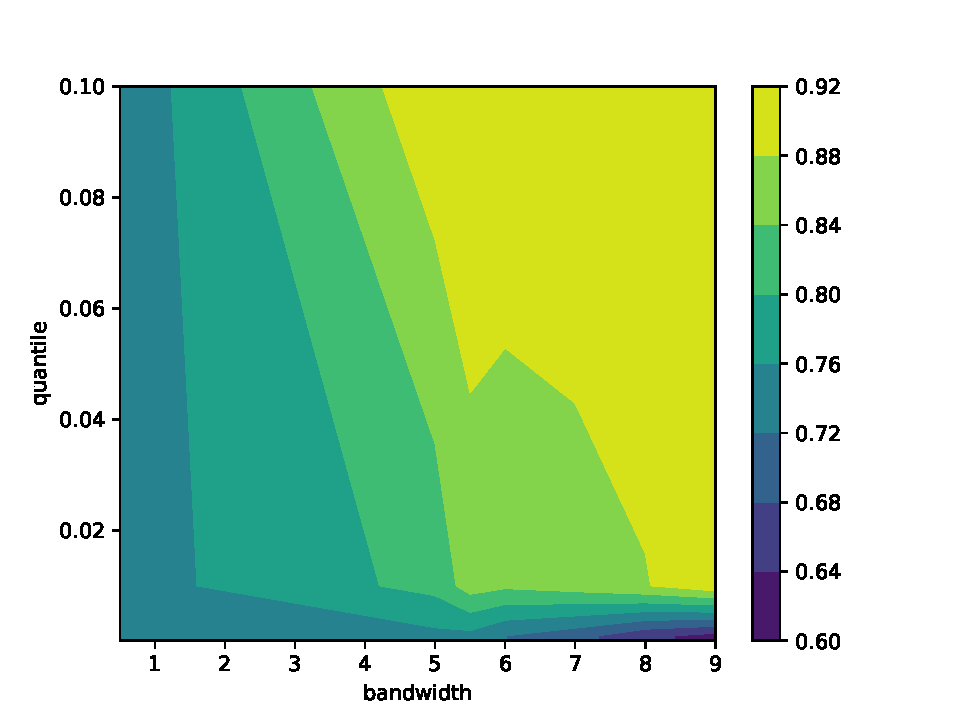
\includegraphics[width=\textwidth]{images/kde-accuracy.pdf}
        \caption{KDE Accuracy}
    \end{minipage}
    \hfill
    \begin{minipage}[t]{0.5\textwidth}
        \vspace{0pt}
        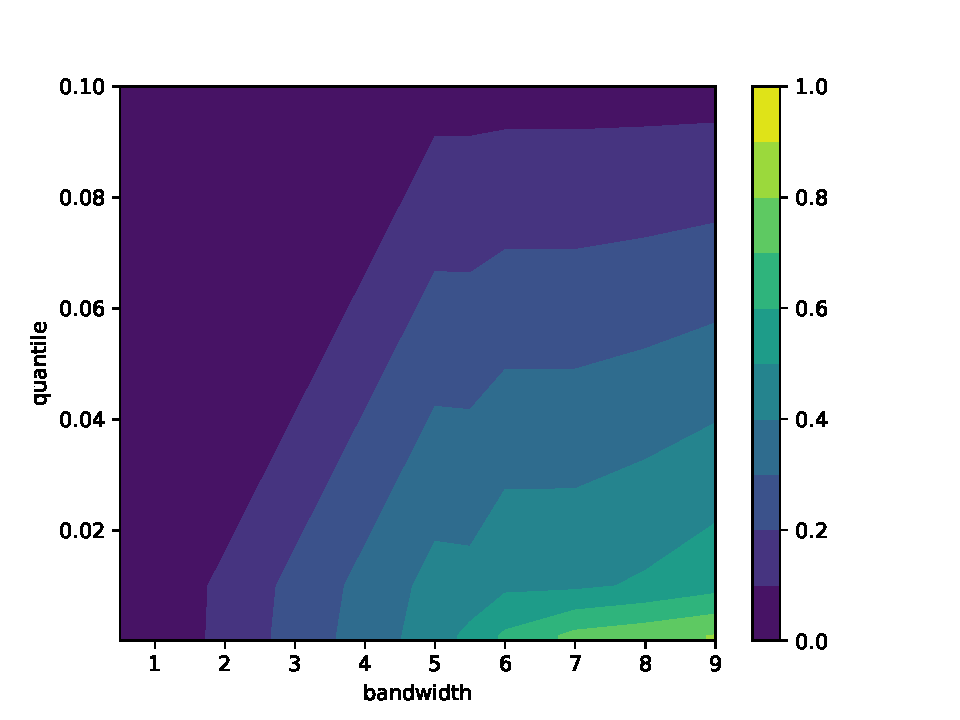
\includegraphics[width=\textwidth]{images/kde-precision.pdf}
        \caption{KDE Precision}
    \end{minipage}
    \\
    \begin{minipage}[t]{0.5\textwidth}
        \vspace{0pt}
        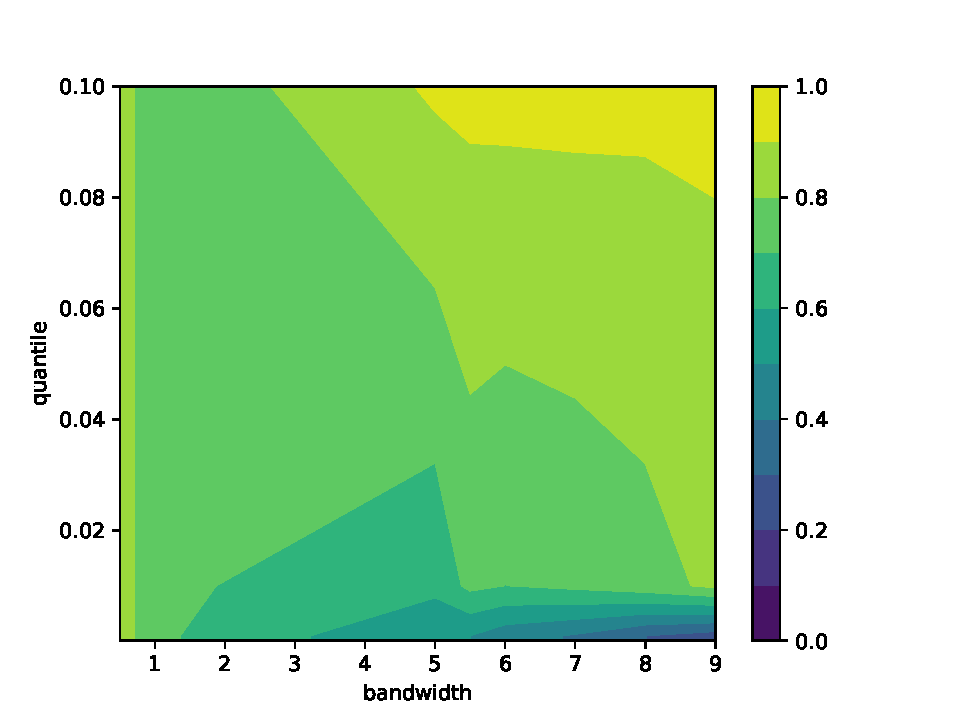
\includegraphics[width=\textwidth]{images/kde-recall.pdf}
        \caption{KDE Recall}
    \end{minipage}
    \hfill
    \begin{minipage}[t]{0.5\textwidth}
        \vspace{0pt}
        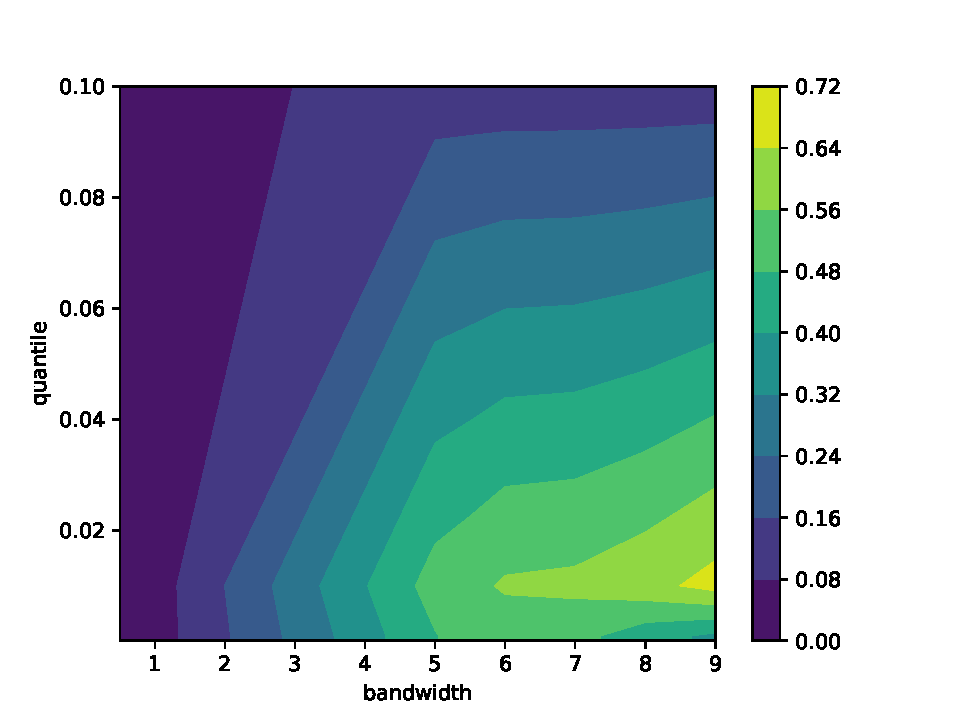
\includegraphics[width=\textwidth]{images/kde-f1.pdf}
        \caption{KDE F1 score}
    \end{minipage}
\end{figure}

\noindent

\section{Modele supervizate}

\subsection{SVM Supervizat}

Pentru a profita de faptul că avem la dispoziţie etichetele datelor, vom trata 
problema şi din punct de vedere supervizat. \textcolor{blue}{Scopul acestui experiment
este de a vedea impactul etichetelor asupra performanţei algoritmilor, 
comparând cazul ideal, unde putem folosi metode supervizate, cu cel din lumea reală,
unde, de obicei, ne bazăm pe cele nesupervizate în lipsa etichetelor.}

Gaussian Mixture Model şi Kernel 
Density Estimation nu pot fi aplicate decât într-un mediu nesupervizat, aşa 
că vom antrena doar SVM-ul, dar de data aceasta pentru clasificare binară.
Astfel, putem observa performanţa algoritmilor prezentaţi anterior şi faţă 
de un algoritm supervizat care are de rezolvat o problemă relativ mai uşoară.

O modificare pe care o vom face la modul de împărţire al setului de date 
este că de această dată stratificarea este luată în calcul, aşa că păstrăm 
ponderile claselor aproximativ la fel în toate cele 3 partiţii.

Şi aici, kernel-ul Gaussian este cel care oferă cele mai bune rezultate cu 
valori scăzute pentru $\gamma$, similar cu cazul OCSVM, dar parametrul 
$\nu$ este înlocuit
de parametrul $C$ care are rolul de regularizare în SVM-ul Soft-Margin.

Se observă o creştere substanţială a valorilor metricilor atunci când tratăm 
problema în mod supervizat, \textbf{F1 Score} 
depăşind 0.87 pe setul de validare, în timp ce 
OCSVM pe setul de validare abia atingea 0.66.

\begin{table}[H]
    \centering
    \begin{tabularx}{\textwidth}{
        |X
        |X
        |X
        |X
        |X
        |X|
    }
    \hline
    $\gamma$ & $C$ & {Accuracy} & {Recall} & {Precision} & {F1 Score} \\
    \hline
    \rowcolor{gray!20} 0.01 & 0.1 & 0.7972 & 0.5946 & 0.8302 & 0.6929 \\
    0.01 & 0.5 & 0.9053 & 0.8108 & 0.8571 & 0.8333 \\
    \rowcolor{gray!20} 0.01 & 1.0 & 0.9053 & 0.8108 & 0.8824 & 0.8451 \\
    0.01 & 2.0 & 0.9053 & 0.8108 & 0.8955 & 0.8511 \\
    \rowcolor{gray!20} 0.01 & 3.0 & 0.9054 & 0.8108 & 0.9375 & 0.8696 \\
    \rowcolor{red!40} 0.01 & 4.0 & 0.9054 & 0.8108 & 0.9524 & 0.8759 \\
    \rowcolor{gray!20} 0.02 & 0.1 & 0.7094 & 0.4189 & 0.7750 & 0.5439 \\
    0.02 & 0.5 & 0.8850 & 0.7703 & 0.8769 & 0.8201 \\
    \rowcolor{gray!20} 0.02 & 1.0 & 0.8918 & 0.7838 & 0.9355 & 0.8529 \\
    0.02 & 2.0 & 0.8919 & 0.7838 & 0.9508 & 0.8593 \\
    \rowcolor{gray!20} 0.02 & 3.0 & 0.8919 & 0.7838 & 0.9508 & 0.8593 \\
    0.02 & 4.0 & 0.8919 & 0.7838 & 0.9667 & 0.8657 \\
    \rowcolor{gray!20} 0.03 & 0.1 & 0.6148 & 0.2297 & 0.8947 & 0.3656 \\
    0.03 & 0.5 & 0.8243 & 0.6486 & 0.9412 & 0.7680 \\
    \rowcolor{gray!20} 0.03 & 1.0 & 0.8783 & 0.7568 & 0.9492 & 0.8421 \\
    0.03 & 2.0 & 0.8851 & 0.7703 & 0.9661 & 0.8571 \\
    \rowcolor{gray!20} 0.03 & 3.0 & 0.8851 & 0.7703 & 0.9661 & 0.8571 \\
    0.03 & 4.0 & 0.8851 & 0.7703 & 0.9661 & 0.8571 \\
    \hline
    \end{tabularx}
    \caption{Grid Search pentru SVM}
\end{table}
  
\chapter{Compararea modelelor finale}

În final, antrenăm fiecare tip de model cu hiperparametrii optimi găsiţi 
folosind setul de validare şi folosim setul de testare pentru a evalua
imparţial modelele finale.

\begin{table}[H]
    \centering
    \begin{tabularx}{\textwidth}{
        |X
        |X
        |X
        |X
        |X|
    }
    \hline
    {Model} & {Accuracy} & {Recall} & {Precision} & {F1 Score} \\
    \hline
    \rowcolor{gray!20} \text{OCSVM} & 0.817 & 0.638 & 0.585 & 0.610 \\
    \text{GMM} & 0.865 & 0.735 & 0.505 & 0.599 \\
    \rowcolor{gray!20} \text{KDE} & 0.863 & 0.731 & 0.502 & 0.596 \\
    \hline
    \end{tabularx}
    \caption{Performanţa fiecărui model pe setul de testare}
\end{table}

Cele 2 modele care au o performanţă similară sunt Gaussian Mixture Model și Kernel Density Estimation,
ultimul având o valoare puţin mai mică pentru F1 score faţă de cel din urmă, dar cu un timp de antrenare 
mult mai mare. Kernel Density Estimation este de departe un model nepotrivit 
pentru acest set de date, necesitând un timp crescut de antrenare pentru 
niște rezultate mediocre. 

Precision este scăzut şi prin urmare şi 
f1 score este scăzut. În schimb, recall are o valoare mai ridicată pentru toate modelele. Acest 
fapt ne arată că detectăm o cantitate mare de anomalii, dar în acelaşi timp, semnalăm un număr 
mare de tranzacţii obişnuite ca fiind frauduloase. Acest lucru poate deveni un inconvenient 
pentru client în cazul în care tranzacţia este anulată ca urmare a raportării incorecte.

Gaussian Mixture Model a fost modelul cu valoarea cea mai mare pentru f1 score
pentru setul de validare, chiar dacă nu este 
un model la fel de complex precum celelalte 2 tehnici nesupervizate. De asemenea, 
acesta a necesitat doar 3 minute pentru
antrenare şi prezicere a etichetelor, dar a produs rezultate mai bune decât
One class SVM şi decât Kernel Density Estimation care au avut nevoie de o perioada
îndelungată pentru antrenare şi căutare a hiperparametrilor optimi.

Totuşi, pe setul de test, One Class SVM este cel care obţine cel mai mare f1 score.

Ilustrăm şi ROC Curve alături de metrica AUC pentru modelele finale. Cu cât graficul 
tinde să se lipească de colţul stânga sus, cu atât aria de sub grafic creşte rezultând 
într-o performanţă mai bună. Linia punctată pe diagonală 
din fiecare diagramă reprezintă graficul produs de clasificatorul aleatoriu şi are rolul
de a marca marginea inferioară a performanţei faţă de această metrică. De asemenea, este 
de menţionat că dacă graficul se află sub linia diagonală, atunci am trage concluzia că
algoritmul nostru este inutil. Totuşi, putem inversa clasa negativă cu cea pozitivă şi 
astfel obţinem simetricul graficului faţă de diagonală care acum, evident, se află deasupra
liniei. Prin urmare, distanţa între grafic şi linie este o măsură mai relevantă decât poziţia
relativă. Se presupune că operaţia de aplicare a simetricului este folosită unde este cazul 
pentru diagramele de mai jos.

ROC Curve are nevoie ori de probabilităţi ori de valori ce exprimă încrederea pentru fiecare 
prezicere, fără aplicarea vreunui prag. Kernel Density Esimation şi Gaussian Mixture Model 
produc deja probabilităţi, pe când One Class SVM nu produce decât distanţa faţă de hiperplanul
de separare. Totuşi, vom folosi un truc pentru a transforma rezultatele OCSVM în valori 
de încredere \cite{stackoverflow-auc}. Înlocuim fiecare valoare cu valoarea respectivă scăzută din valoarea maximă
dată de funcţia de decizie după cum urmează:

$$y_{score} = MAX - f(y)$$
unde 

\begin{itemize}
    \item $y_{score}$ este valoarea folosită pentru ROC Curve
    \item $MAX$ este $\max_{i=1}^{n} f(y_{i})$ pentru $n$ observaţii
    \item $f$ este funcţia de decizie 
\end{itemize}

Astfel, putem compara modelele finale folosind şi metrica AUC care ne 
indică cât de robust este un model, indiferent de pragul ales pentru 
o anumită problemă. Clasamentul este acelaşi şi aici,
cu One Class SVM fiind cel mai performant, urmat de Gaussian Mixture
Model, iar Kernel Density Estimation la coadă.

În concluzie, \textbf{One Class SVM} este modelul cel mai bun cu \textbf{f1 score}
de 0.61 şi 
\textbf{AUC} de 0.91 pe setul de test, 
dar Gaussian Mixture Model este şi el un candidat
bun datorită vitezei de antrenare şi inferenţă.

\begin{figure}[!htb] % Use a separate page for the figure
    \begin{minipage}[t]{0.5\textwidth}
        \vspace{0pt}
        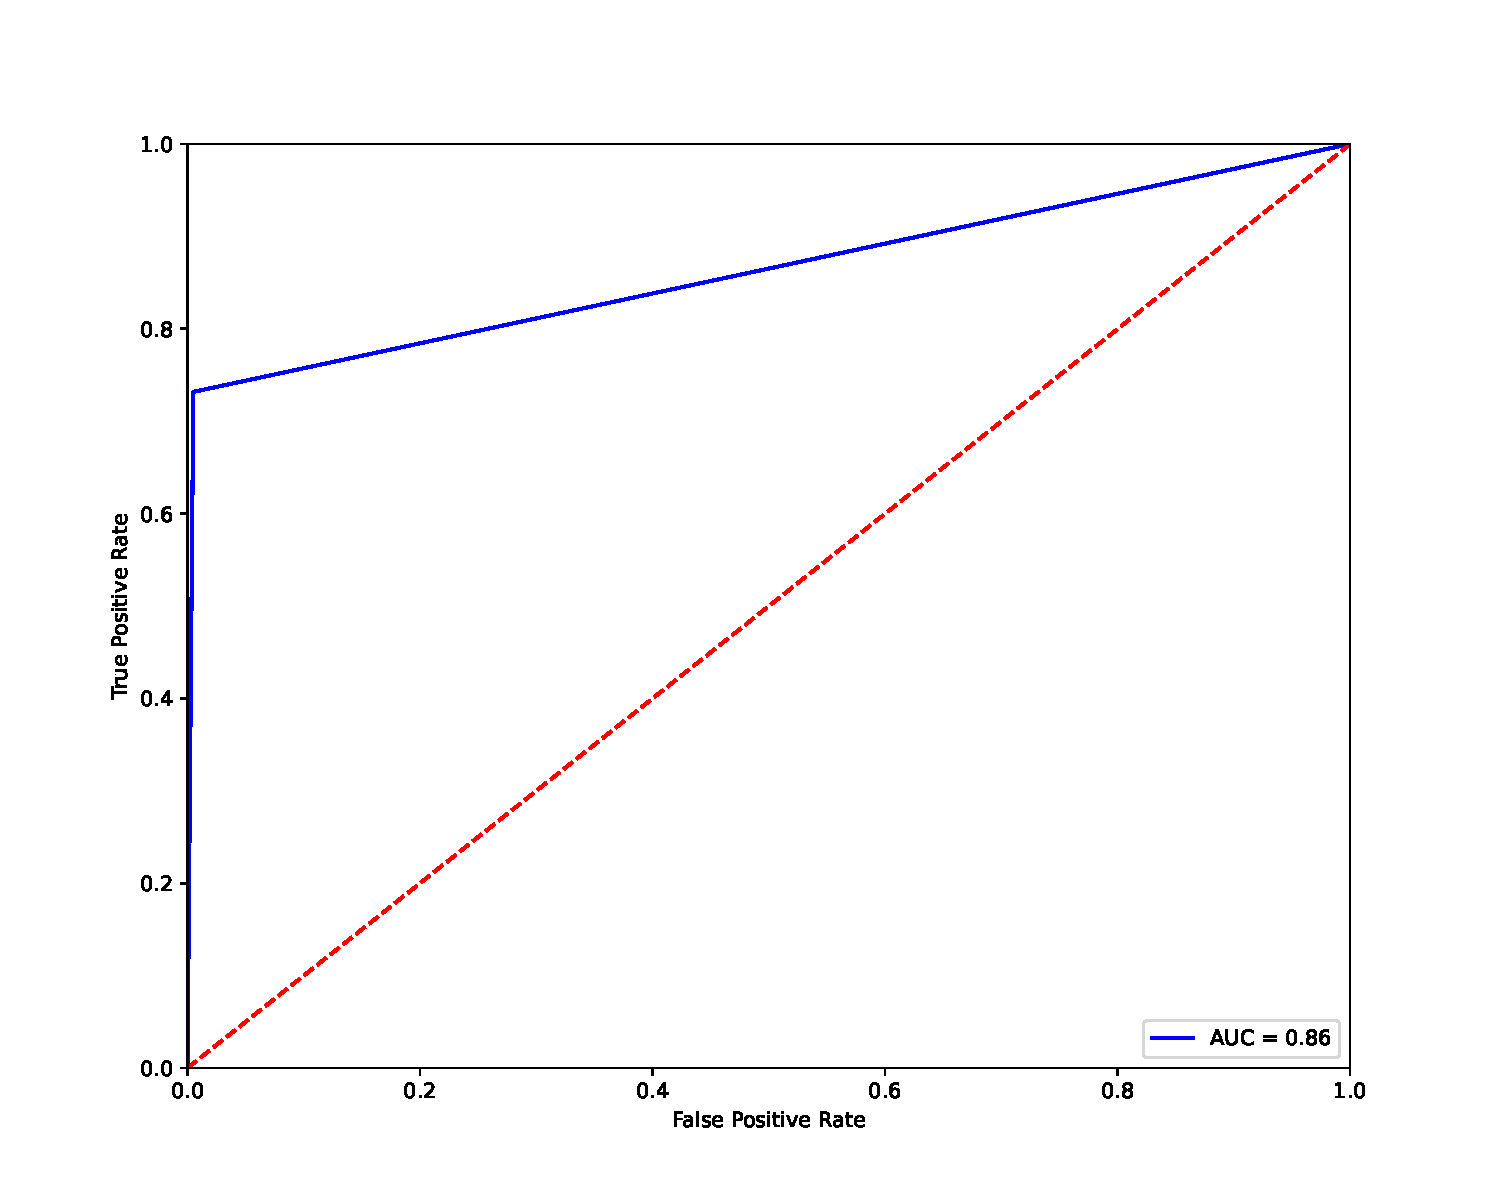
\includegraphics[width=\textwidth]{images/kde-roc.pdf}
        \caption{ROC Curve KDE} 
    \end{minipage}
    \hfill
    \begin{minipage}[t]{0.5\textwidth}
        \vspace{0pt}
        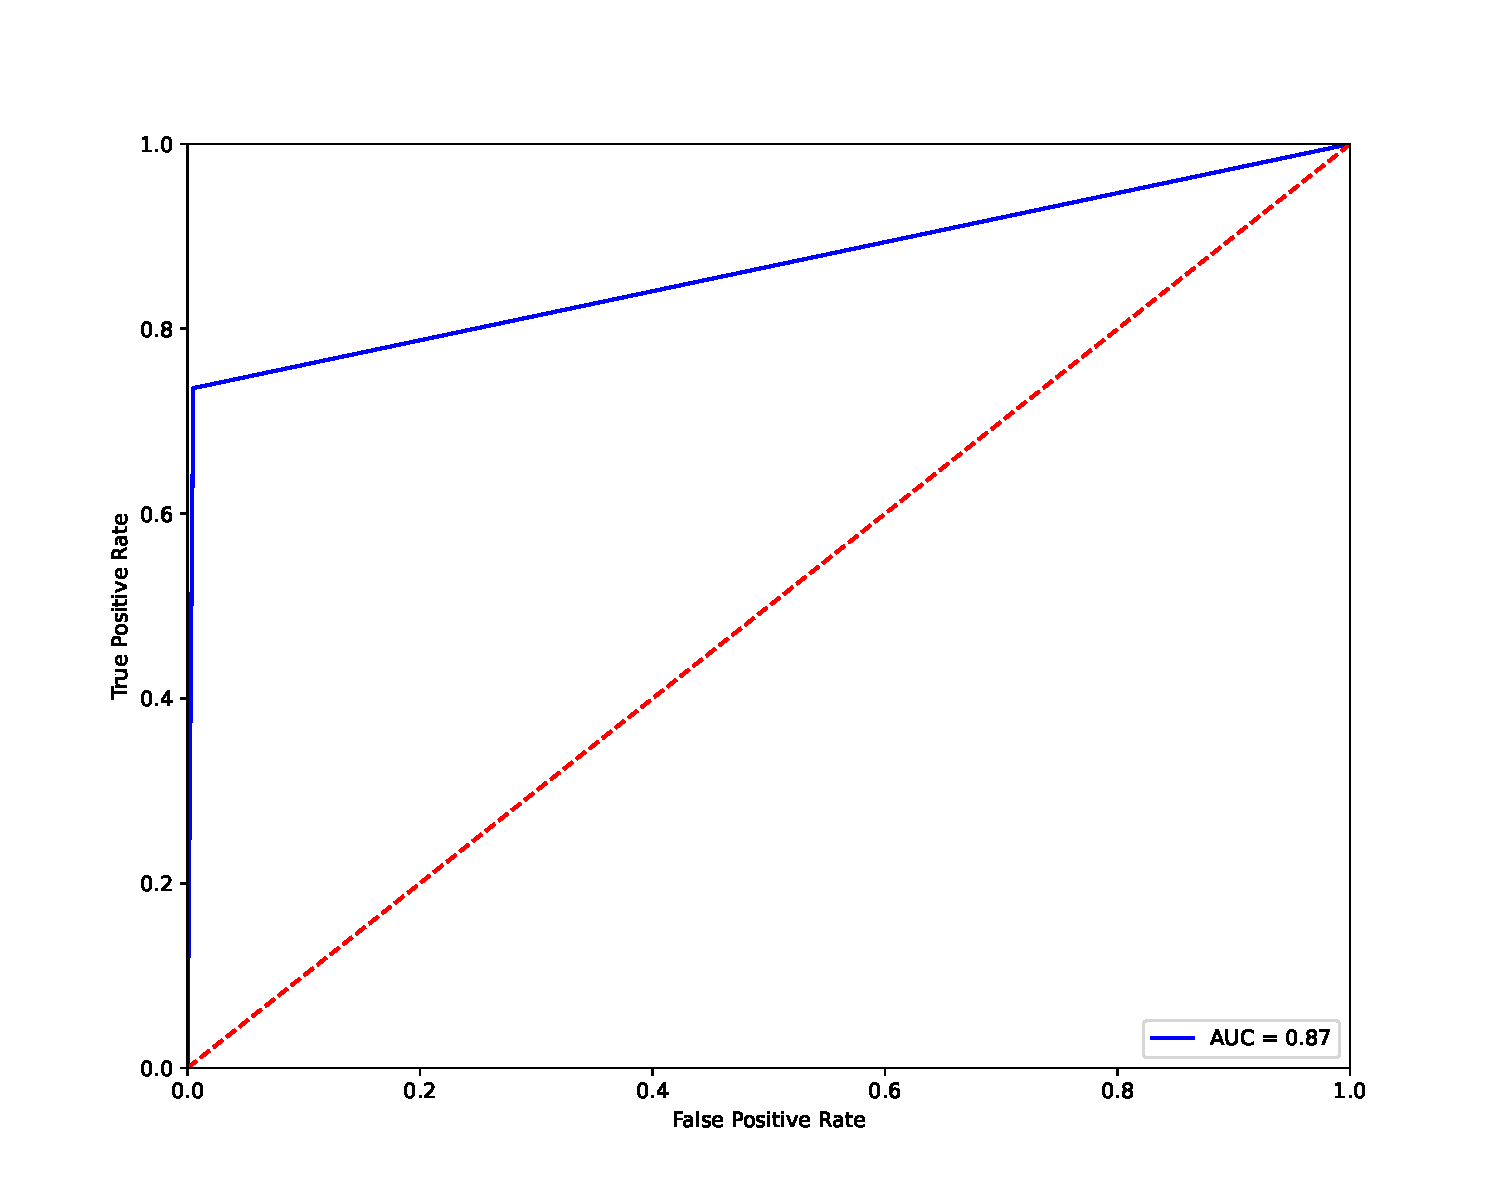
\includegraphics[width=\textwidth]{images/gmm-roc.pdf}
        \caption{ROC Curve GMM}
    \end{minipage}
    
    \begin{minipage}[t]{1\textwidth}
       \centering
        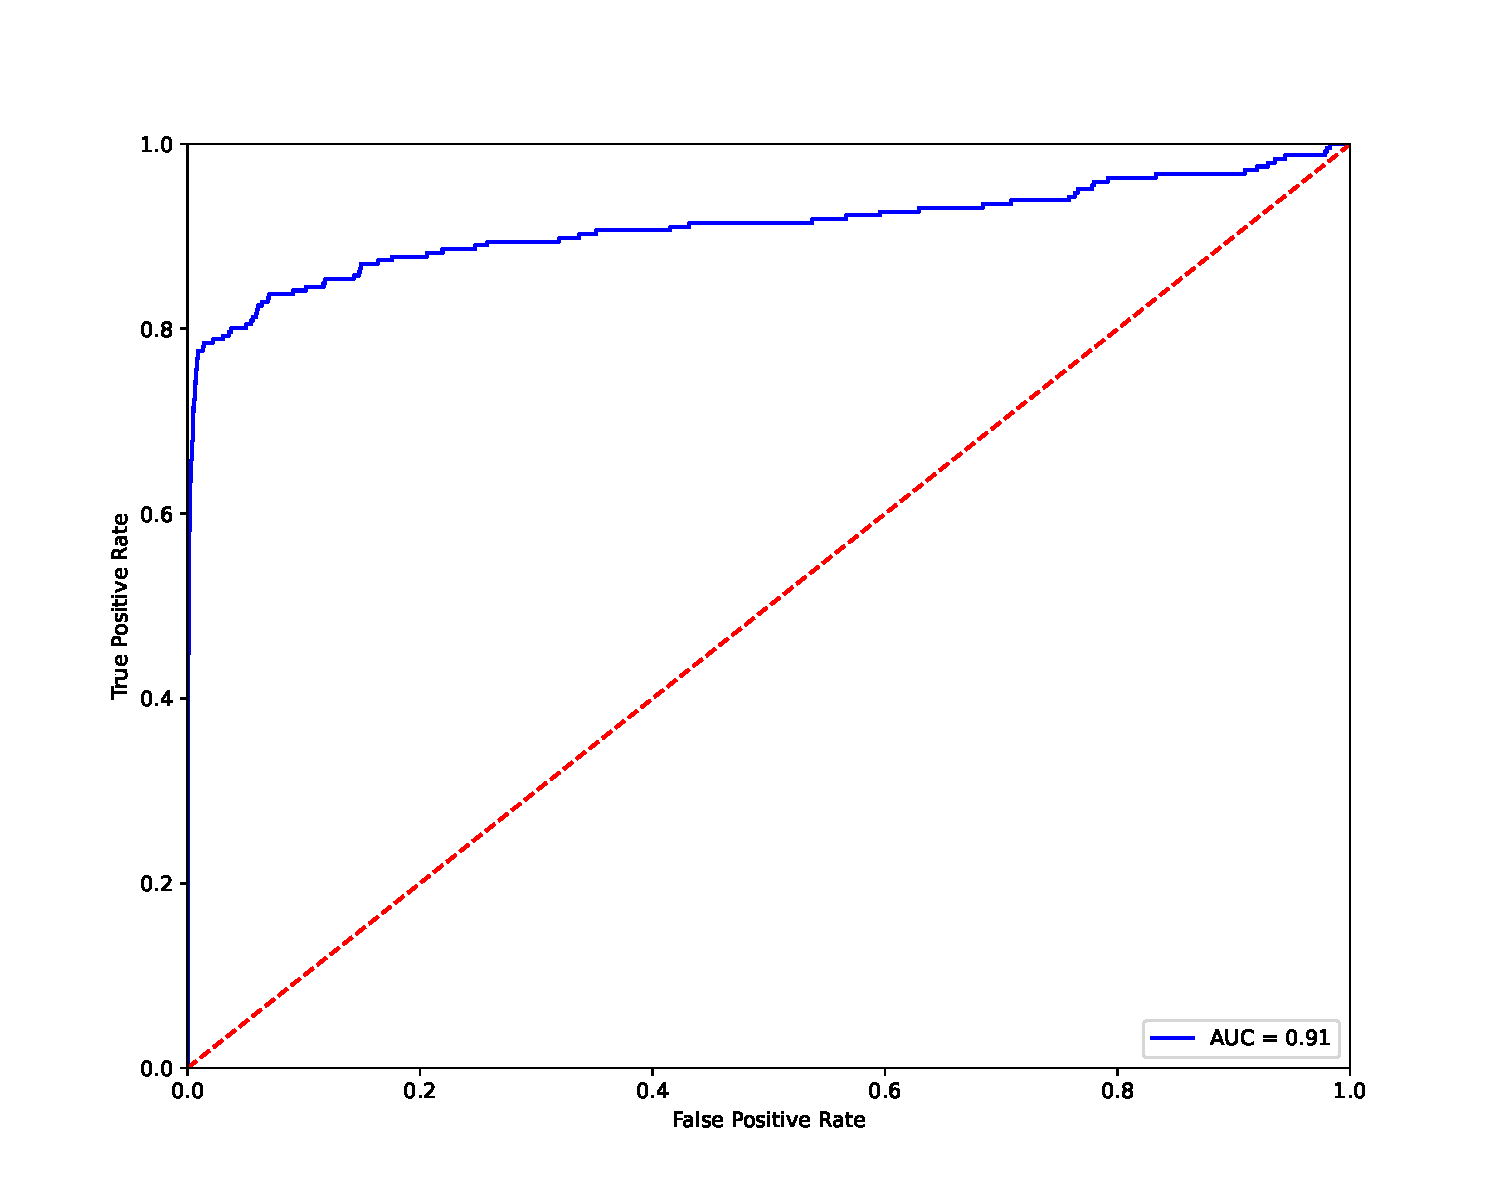
\includegraphics[width=\textwidth]{images/ocsvm-roc.pdf}
        \caption{ROC Curve OCSVM}
    \end{minipage}
    
\end{figure}

\noindent
\chapter{Concluzii}

În această lucrare am ilustrat una din multitudinea de aplicaţii în industrie a 
detecţiei anomaliilor, anume identificarea tranzacţiilor frauduloase. Am explorat un 
set de date adnotat cu informaţii despre tranzacţii bancare şi am arătat cum putem evalua
performanţa unor metode de învăţare automată nesupervizată folosind metrici din domeniul 
învăţării supervizate, mai specific, clasificarea binară.

Deşi tehnicile folosite aparţin învăţarii nesupervizate, am arătat cum putem exploata
cunoştinţele din alte două categorii, anume semi-supervizată şi supervizată. 

Prima a fost 
utilă pentru faptul că am antrenat algoritmi pe un set de date mare fără să utilizăm 
etichetele punctelor, dar apoi am folosit un set de date cu o mărime relativă mult mai mică
pentru a analiza performanţa algoritmilor. 

A doua a fost de folos pentru că ne-a oferit 
o multitudine de metrici care într-un context strict nesupervizat nu ar fi existat, fiind 
nevoie de inspecţia unui om pentru analiză.

Alegerea metricilor corespunzătoare
este probabil una din cele mai dificile părţi atunci când căutăm o soluţie eficientă pentru 
problema dată, mai ales când proporţia de clase este neechilibrată şi acordăm o importanţă mai 
mare unei clase faţă de cealaltă, întrucât o alegere greşită ne poate induce în eroare cu privinţă
la utilitatea reală a algoritmului, după cum am şi demonstrat.

De asemenea, am analizat trei algoritmi cu caracteristici diferite, dar cu 
scopuri similare, anume idenfiticarea anomaliilor.

One Class SVM se 
foloseşte de un hiperplan de separare pentru a împărţi spaţiul Hilbert într-o porţiune 
care cuprinde toate punctele normale şi una care cuprinde restul punctelor izolate. Astfel,
putem spune că acesta face o clasificare dură a anomaliilor, întrucât ne indică doar daca
o observaţie este normală sau nu. 

La polul opus, avem Gaussian Mixture Model şi Kernel Density 
Estimation care încearcă să estimeze funcţia densitate de probabilitate din care au fost 
generate datele şi să atribuie fiecărei observaţii noi o valoare dată de această funcţie.
Peste aceste probabilităţi se aplică un prag şi abia apoi obţinem etichetele corespunzătoare.
Astfel, putem spune că acestea fac o clasificare slabă a anomaliilor, întrucât ne indică 
cât de probabil este ca punctul să fie normal sau nu, dar nu ne indică concret clasa 
de care aparţine.

Deşi am întâmpinat probleme în ilustrarea graficului ROC Curve pentru algoritmul cu clasificare
dură, am demonstrat cum putem transforma distanţele produse de funcţia de decizie în valori 
de încredere pentru a obţine o clasificare slabă artificială.

La final, am observat că modelele au performat mai mult sau mai puţin la fel, cele mai complexe 
având un dezavantaj când vine vorba de complexitatea de timp.

Cu toate acestea, lucrarea nu a abordat problema seriilor de timp, lucru des întâlnit în practică,
dar care creează o direcţie de cercetare interesantă. Două cerinţe relevante pentru acest 
subiect ar fi prognoza şi clasificarea seriilor de timp. 

Prima se referă la prezicerea evoluţiei
în timp a seriei de date şi este folosită ca suport pentru unele modele ce detectează anomaliile
folosindu-se de deviaţia prognozei faţă de valorile observate. Prognoza se bazează strict pe 
valorile punctelor din şir din contextul precedent şi pe modelul antrenat anterior. Deseori,
se utilizează o fereastră glisantă de mărime unitară pentru a crea contextul şi a prezice 
câte un punct pe rând. Este similar cu abordarea clasică 
din domeniul Procesării Limbajului Natural, unde suntem interesaţi să prezicem cuvântul cel 
mai potrivit pentru continuarea unei propoziţii, spre exemplu. Aici, putem privi cuvintele
din text ca fiind puncte dintr-o serie de timp.

A doua se referă la atribuirea unei categorii pentru diverse subşiruri din seriile de timp.
Astfel, metoda poate fi folosită ori pentru post-procesarea rezultatelor obţinute după 
detecţia anomaliilor pentru a categoriza diferitele valori deviante, ori chiar în cadrul 
modelului cu rolul de a clasifica componentele din seriile de date în grupuri relevante,
implict anomalii sau observaţii normale. Metoda ne aduce aminte de clasica problemă
a clasificării unor puncte dintr-un set de date, întâlnită în contextul învăţării automate
supervizate \cite{time-series}.

\printbibliography[heading=bibintoc]

\end{document}